\pagenumbering{arabic}
%\documentclass[slides]{beamer}
\documentclass[mathserif,10pt]{beamer}
%\documentclass[slides,hyperref={pdfpagelabels=false}]{beamer}
%\documentclass[handout,gray]{beamer}
\usepackage[T1]{fontenc}
\usepackage[utf8]{inputenc}
\usepackage{textcomp}
\usepackage{verbatim}
\usepackage{amsbsy}
\usepackage{multicol}
\usepackage{booktabs} % Make some nice tables
\usepackage{ae,aecompl}

%%%%%%%%%%%% COULEURS %%%%%%%%%%%%%%%%%%%%%%%%%%%

\mode<presentation>
{
  \definecolor{beamerstructure}{RGB}{43,79,112}
  \definecolor{sidebackground}{RGB}{230,242,250}
  \definecolor{CTCC}{RGB}{133,188,228}
  \color{beamerstructure}
  \usetheme{default}
  \usepackage{courier}
  \beamertemplateballitem
\setbeamertemplate{navigation symbols}{}
%\setbeamertemplate{sidebar left}{\thispdfpagelabel{\insertframenumber}}
%\setbeamertemplate{footline}{\quad\insertframenumber}
%\usecolortheme{CTCC}
}
\usebackgroundtemplate{\includegraphics[width=1.02\paperwidth]{../templets/ctcc_general.jpg}}

\title{\\\vspace{1cm} Relativistic effects in chemistry}
%\subtitle{\textcolor{magenta}{My subtitle (if applicable)}}
\author{Stig Rune Jensen}
\institute[CTCC]{\\[-6mm]stig.r.jensen@uit.no\\[6mm]UiT The Arctic University of Norway\\[6mm]
\includegraphics[height=1.5cm]{../templets/uio.pdf}\hspace{1cm} 
\includegraphics[height=1.5cm]{../templets/sff.pdf}\hspace{1cm}
\includegraphics[height=1.5cm]{../templets/uit.pdf}}
\date{Troms\o, March 20th 2014}

\newcommand{\gb}[1]{green!#1!black}
\newcommand{\rb}[1]{red!#1!black}
\newcommand{\bb}[1]{blue!#1!black}
\newcommand{\coleq}{red!60!black}
\newcommand{\du}{\textrm{d}}

\usepackage{multicol}
\newcommand{\mydef}{\stackrel{\text{def}}{\hbox{=}}} 

\begin{document}

\footnotesize
\setlength{\unitlength}{\textwidth}

{
\usebackgroundtemplate{\includegraphics[width=1.02\paperwidth]{../templets/ctcc_forside.jpg}}
\maketitle
}

\begin{frame}
    \frametitle{Relativistic effects in chemistry}
    \begin{columns}
    \begin{column}{.6\textwidth}
	\centering
	\begin{exampleblock}{\it{\small{''These [relativistic effects] give rise to difficulties 
	    only when high-speed particles are involved, and are therefore of \textcolor{red}{no 
	    importance} in the consideration of atomic and molecular structure and ordinary 
	    chemical reactions\dots''}}}
	    \vskip2mm
	    \hspace*\fill{\tiny--- Paul AM Dirac, 1929}
	\end{exampleblock}
    \end{column}
    \begin{column}{.4\textwidth}
	\centering
	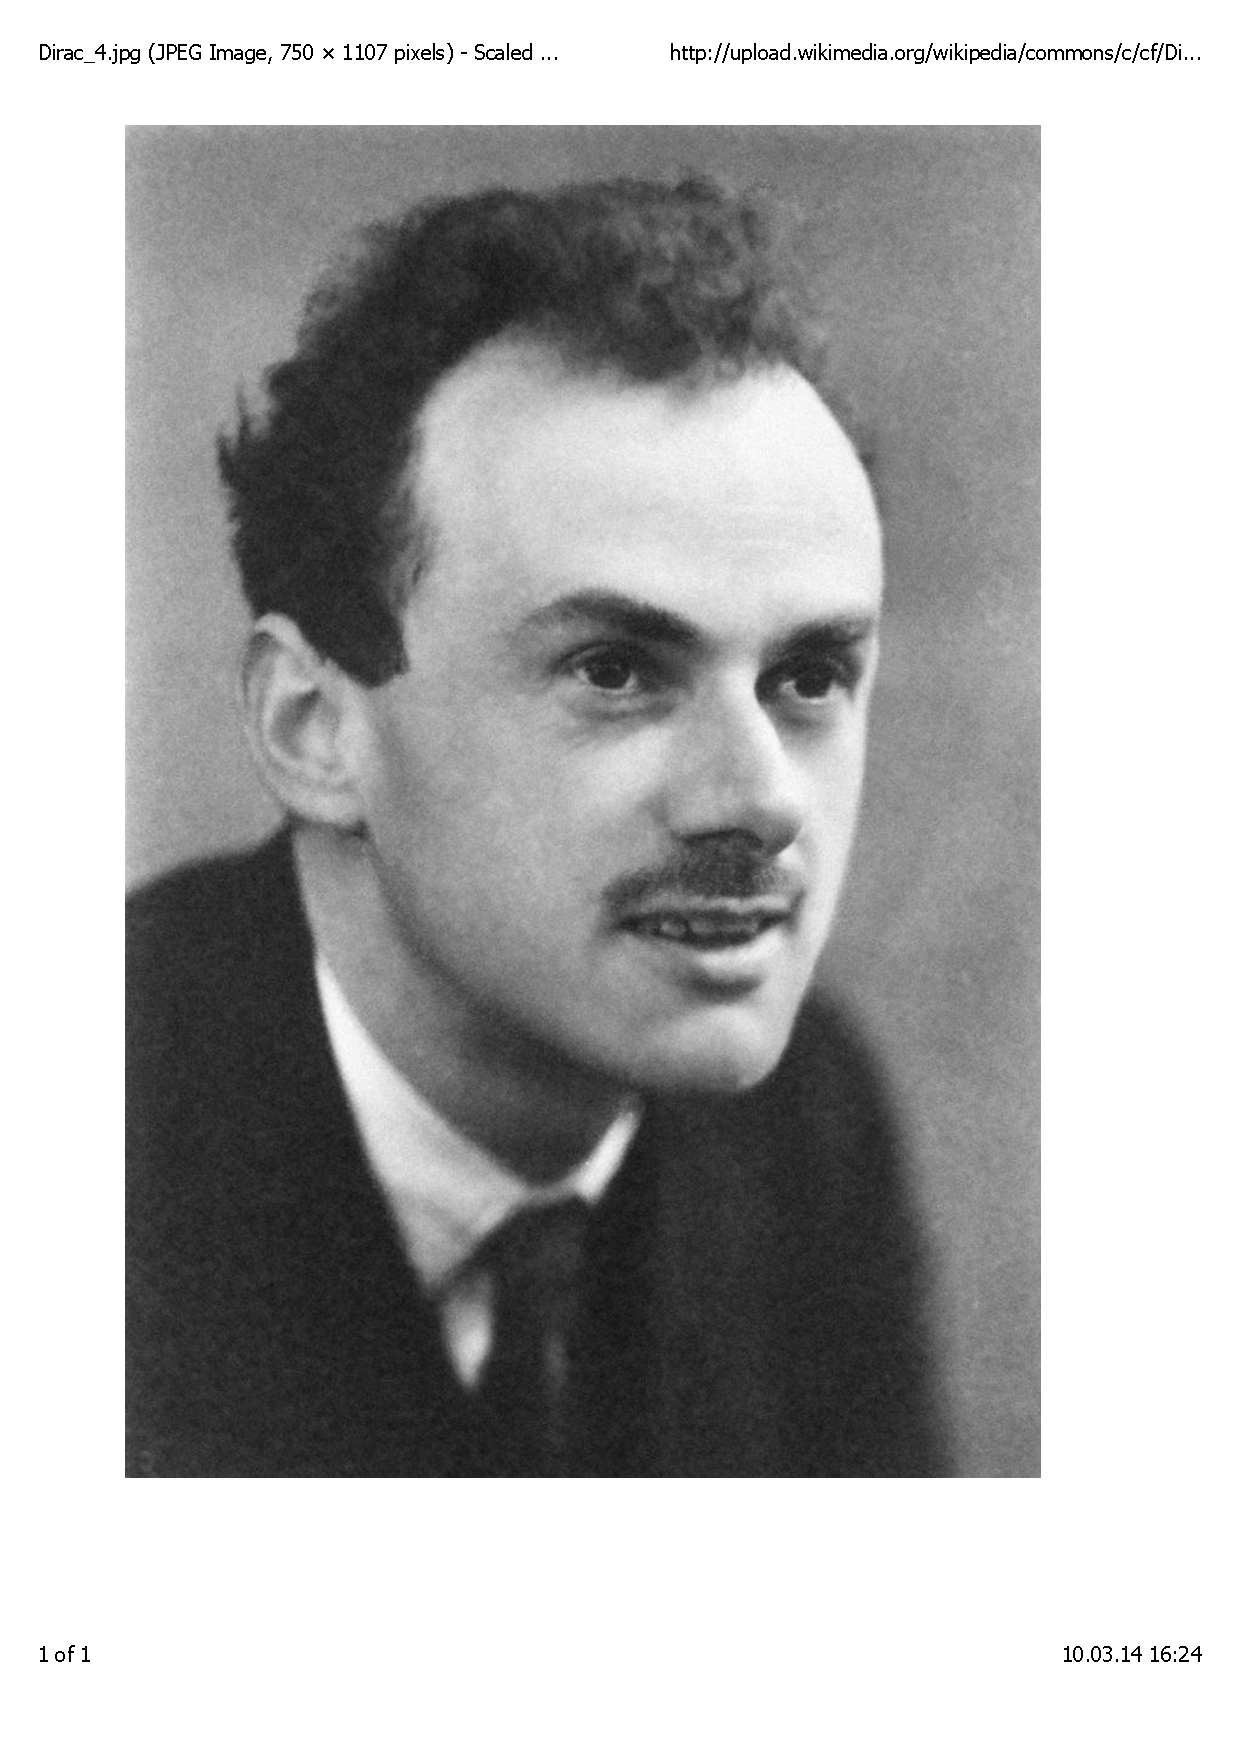
\includegraphics[viewport = 50 200 500 800, clip, scale=0.15]{figures/dirac.pdf}
    \end{column}
    \end{columns}
\end{frame}

\begin{frame}
    \frametitle{Theory of special relativity}
    \begin{columns}
    \begin{column}{.60\textwidth}
	\centering
	\begin{exampleblock}{\it{\small{''Henceforth space by itself, and time by itself,
	    are doomed to fade away into mere shadows, and only a kind of union of the
	    two will perserve an independent reality.''}}}
	    \vskip2mm
	    \hspace*\fill{\tiny--- Hermann Minkowski}
	\end{exampleblock}
    \end{column}
    \begin{column}{.40\textwidth}
	\centering
	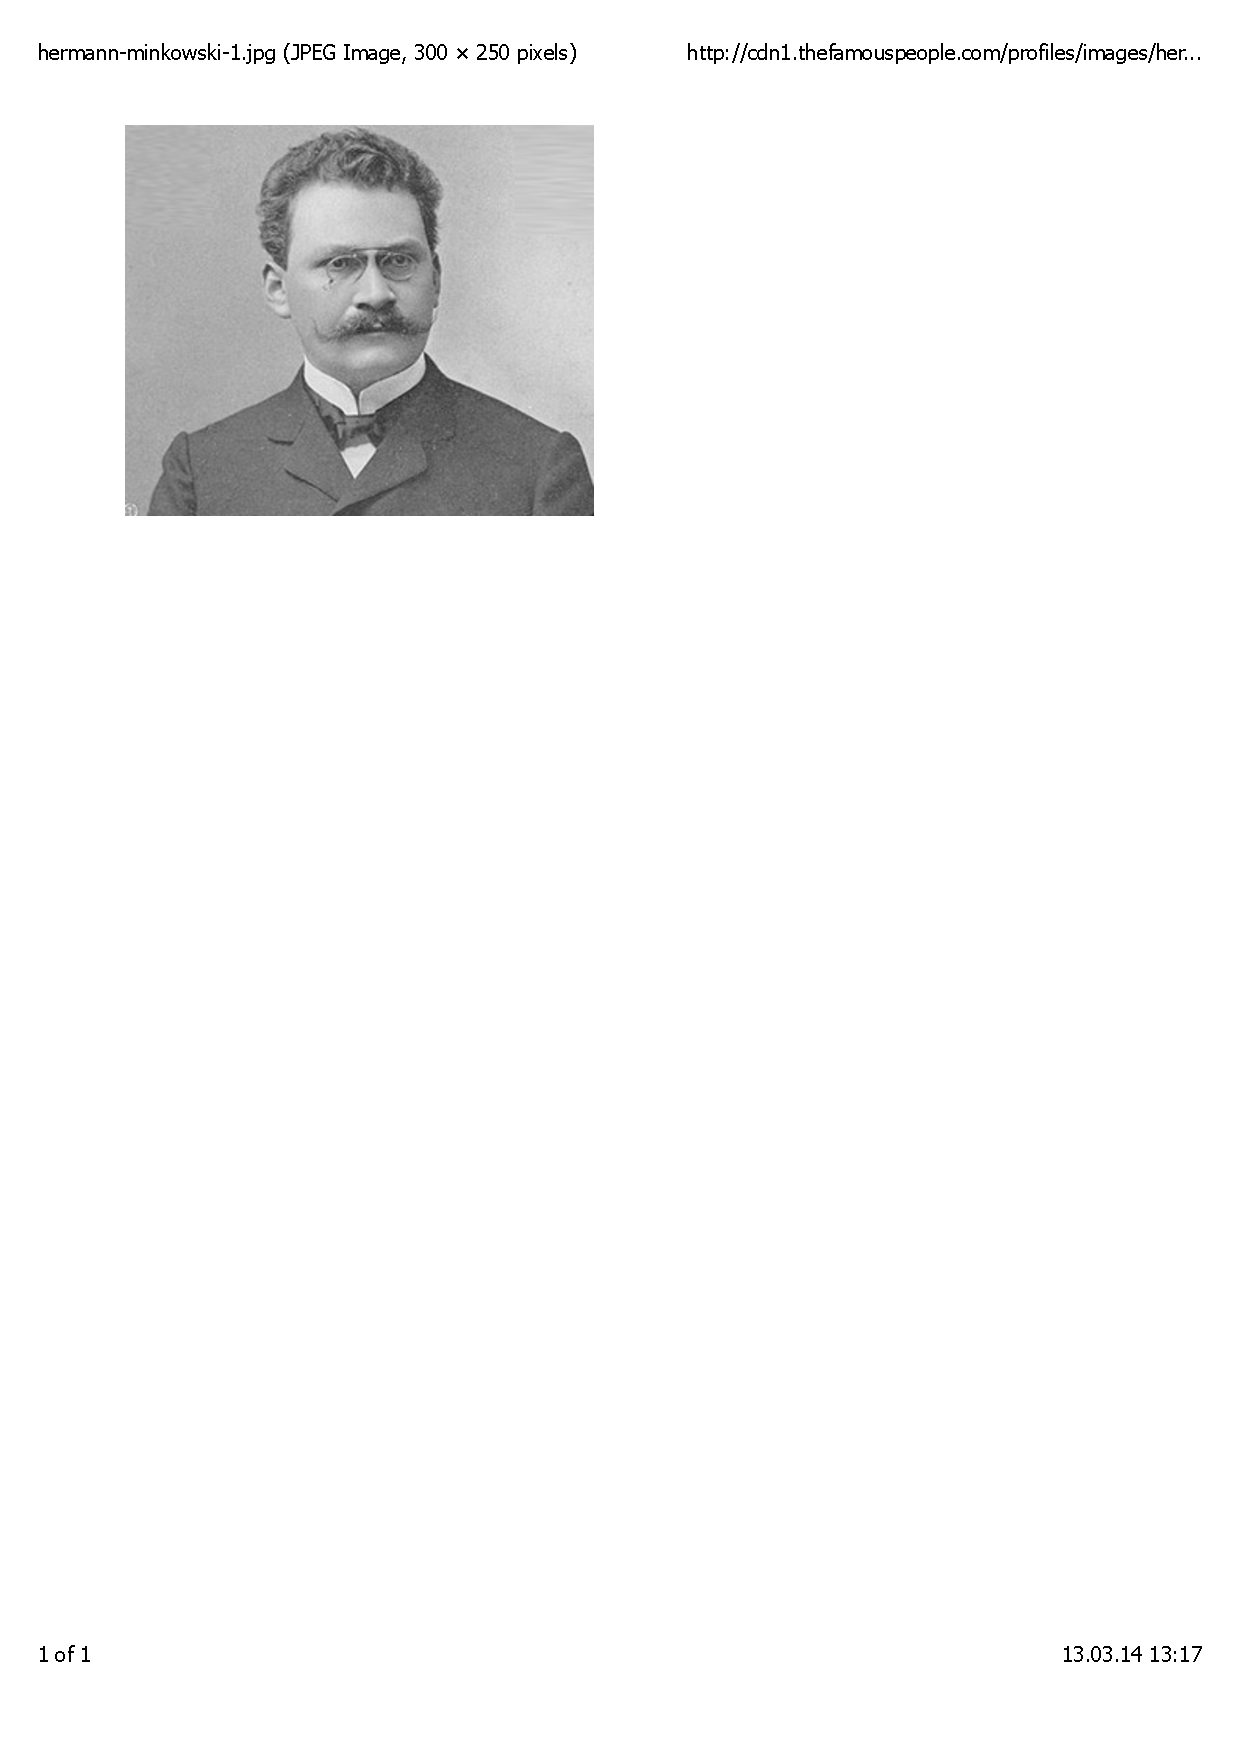
\includegraphics[viewport = 70 600 270 780, clip, scale=0.4]{figures/minkowski.pdf}
    \end{column}
    \end{columns}
    \ \\
    \ \\
    \ \\
    \ \\
    \ \\
    Newtons absolute time and space vs Einstein
\end{frame}

\begin{frame}
    \frametitle{Theory of special relativity}
    \begin{columns}
    \begin{column}{.50\textwidth}
	\begin{itemize}
	\item The speed of light is the same in all reference frames
	\item Remains constant as space and time itself changes
	\begin{equation}
	    \nonumber
	    c = \frac{\Delta x}{\Delta t} = \frac{\Delta x'}{\Delta t'}
	\end{equation}
	\item Lorentz factor
	\begin{equation}
	    \nonumber
	    \gamma = \frac{1}{\sqrt{1-v^2/c^2}}
	\end{equation}
	\item Nothing (particles or information) can move faster than the speed of light
	\end{itemize}
    \end{column}
    \begin{column}{.50\textwidth}
	\centering
	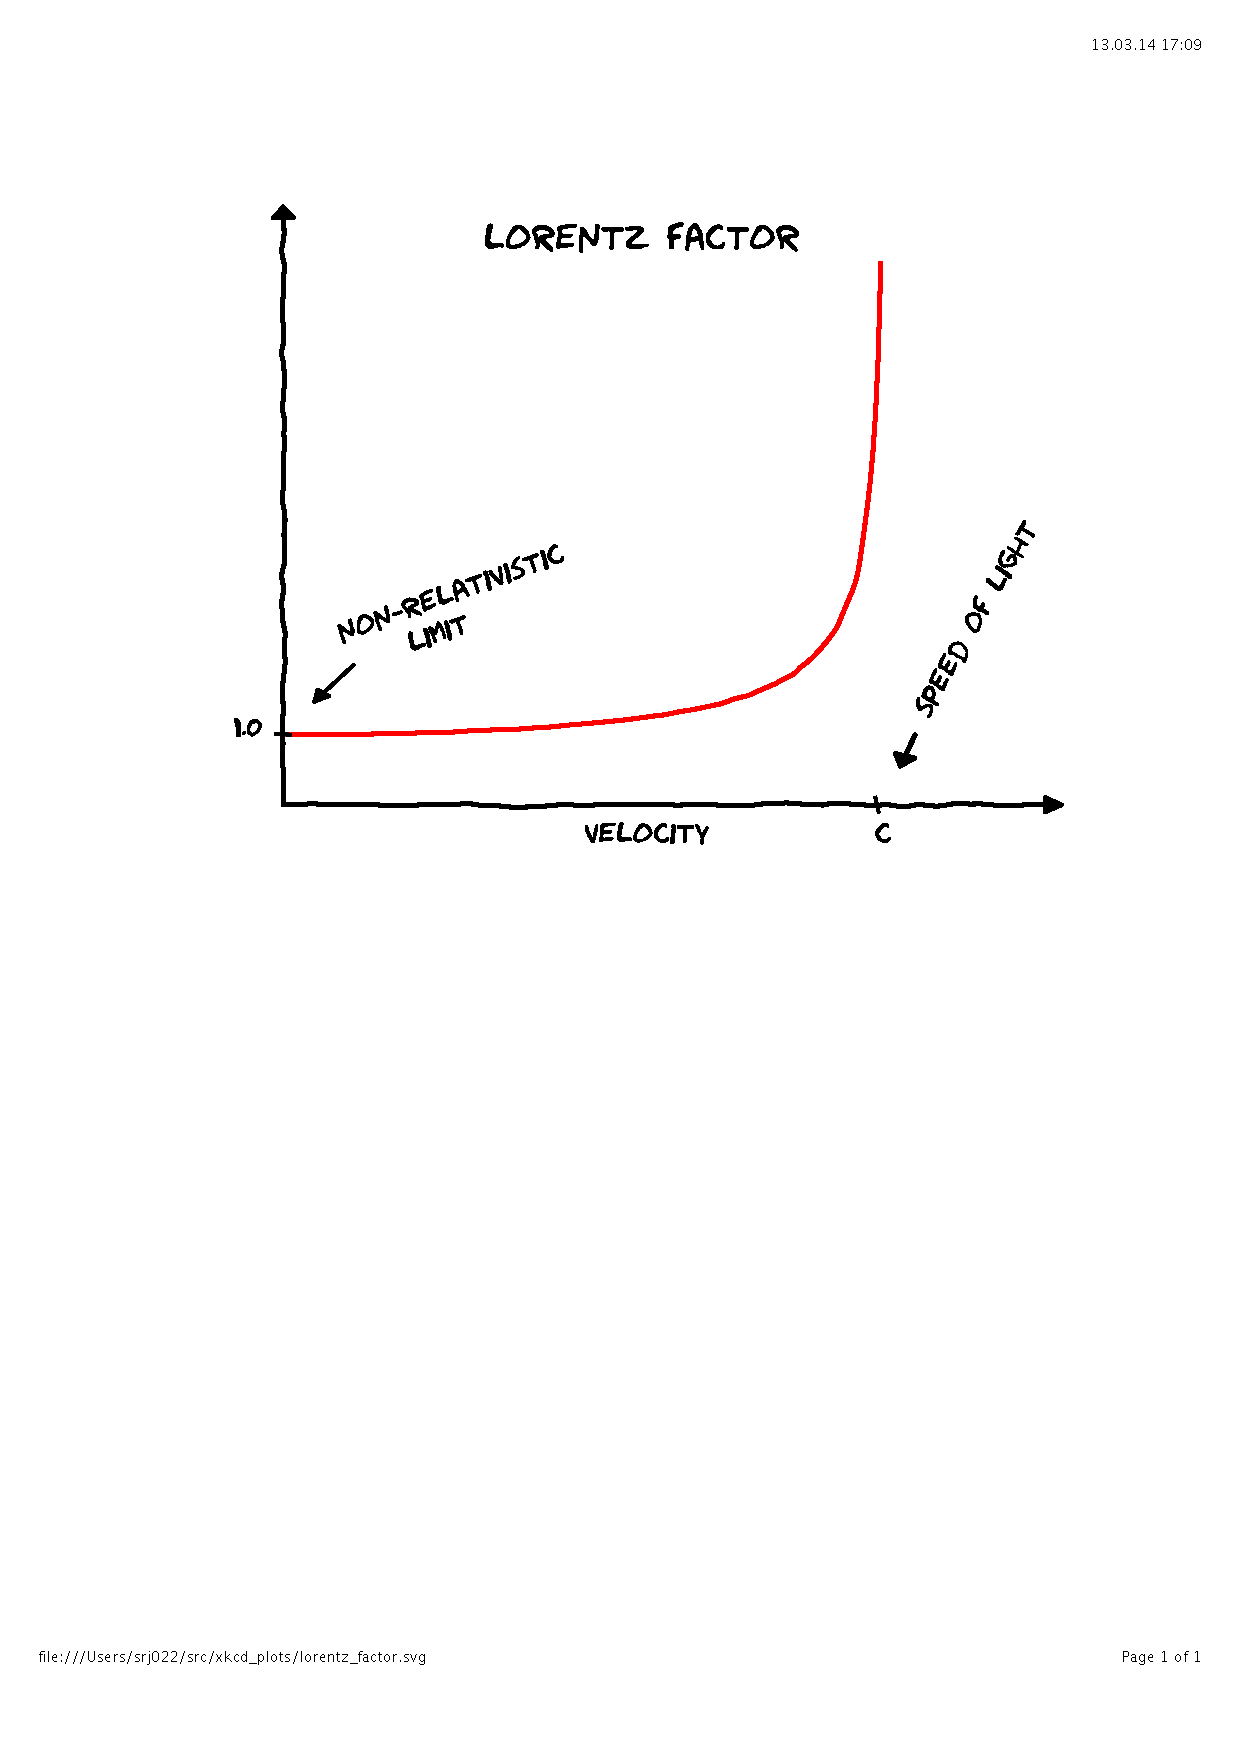
\includegraphics[viewport = 100 400 550 750, clip, scale=0.3]{figures/lorentz_factor.pdf}\\
	\ \\
	\ \\
	\ \\
	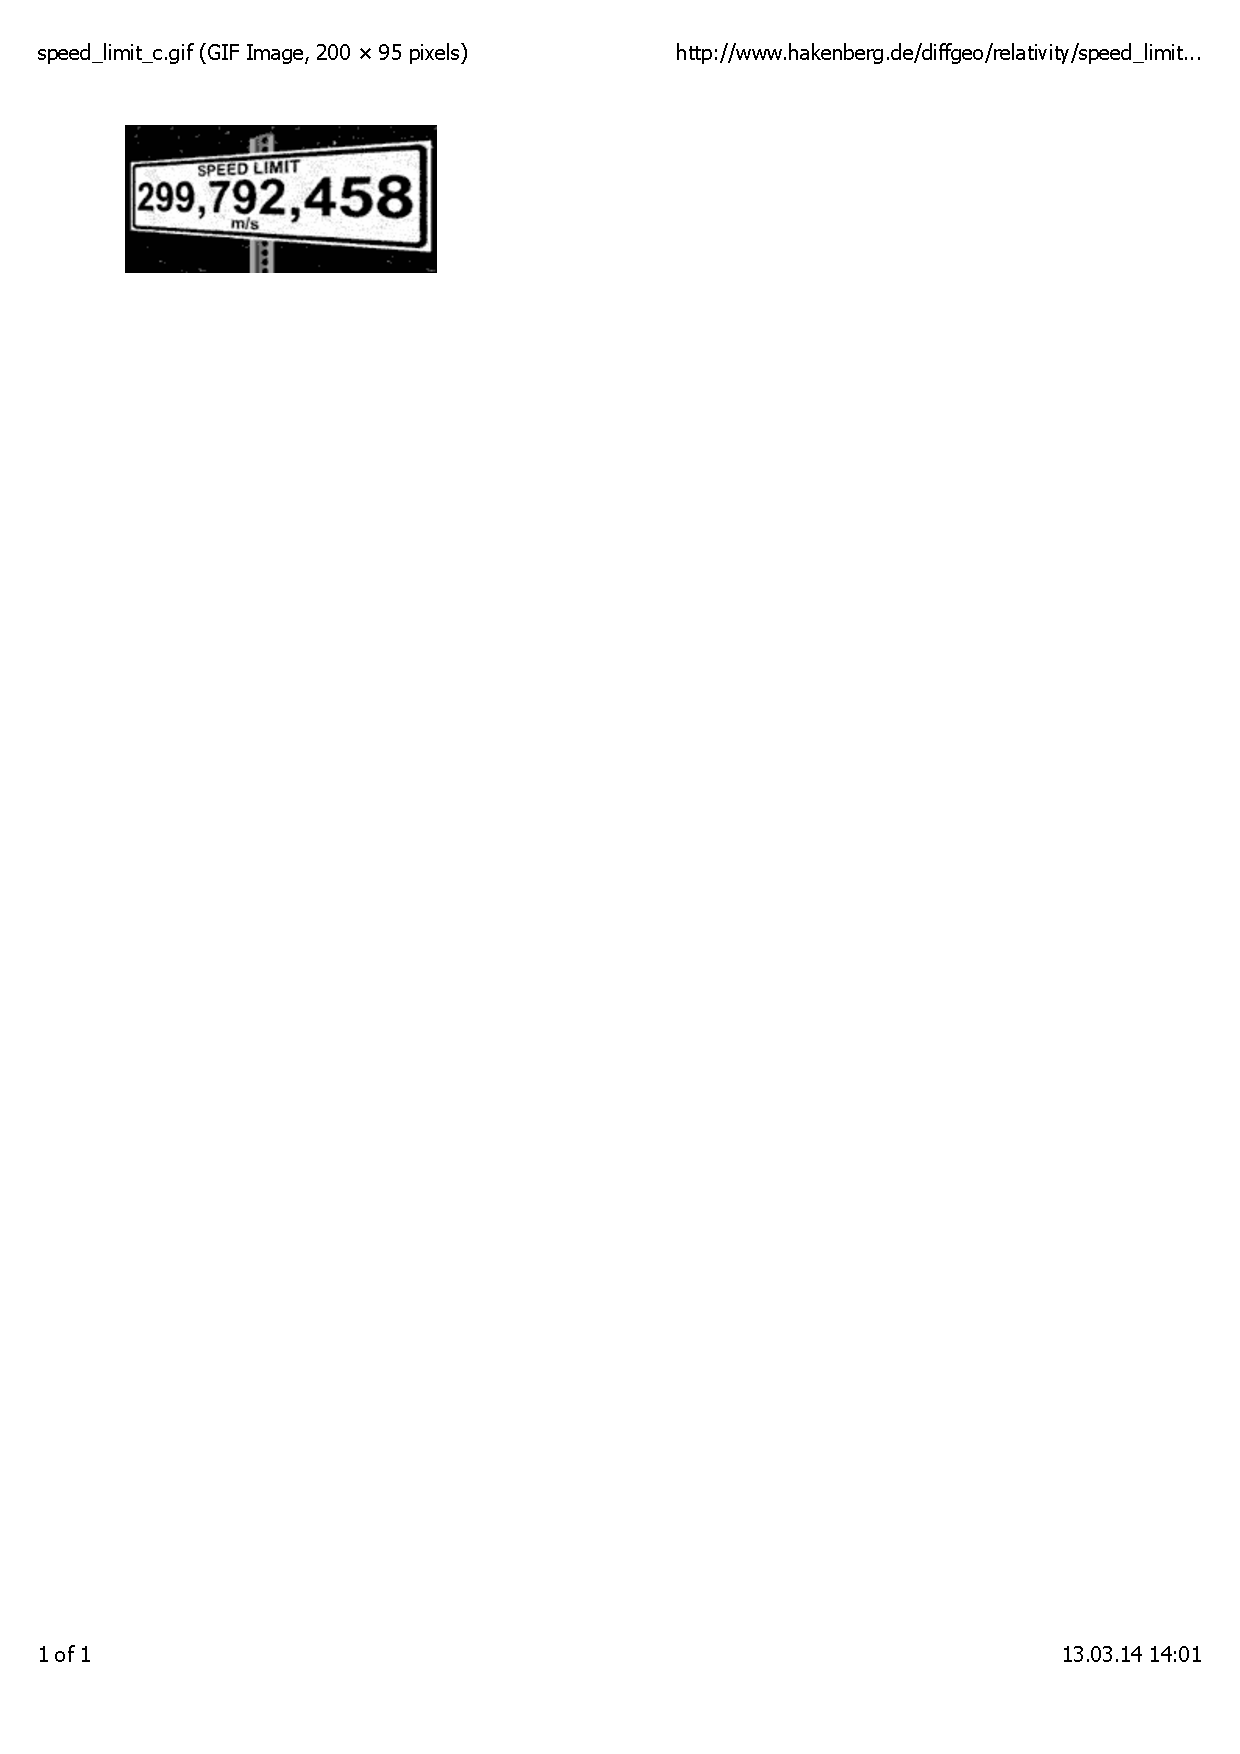
\includegraphics[viewport = 60 710 210 780, clip, scale=0.5]{figures/speed_limit.pdf}
    \end{column}
    \end{columns}
    Four-vectors (momentum, position, velocity, angular momentum, potential, current)
\end{frame}

\begin{frame}
    \frametitle{Relativistic effects in physics}
    \begin{columns}
    \begin{column}{.40\textwidth}
    \begin{itemize}
	\item Mass increase
	    \begin{equation}
		\nonumber
		m_{rel} = \gamma m_0
	    \end{equation}
	\item Length contraction
	    \begin{equation}
		\nonumber
		x_{rel} = \frac{x_0}{\gamma}
	    \end{equation}
	\item Time dilation
	    \begin{equation}
		\nonumber
		t_{rel} = \gamma t_0
	    \end{equation}
	\item Simultaneity is relative
    \end{itemize}
    \end{column}
    \begin{column}{.60\textwidth}
	\centering
	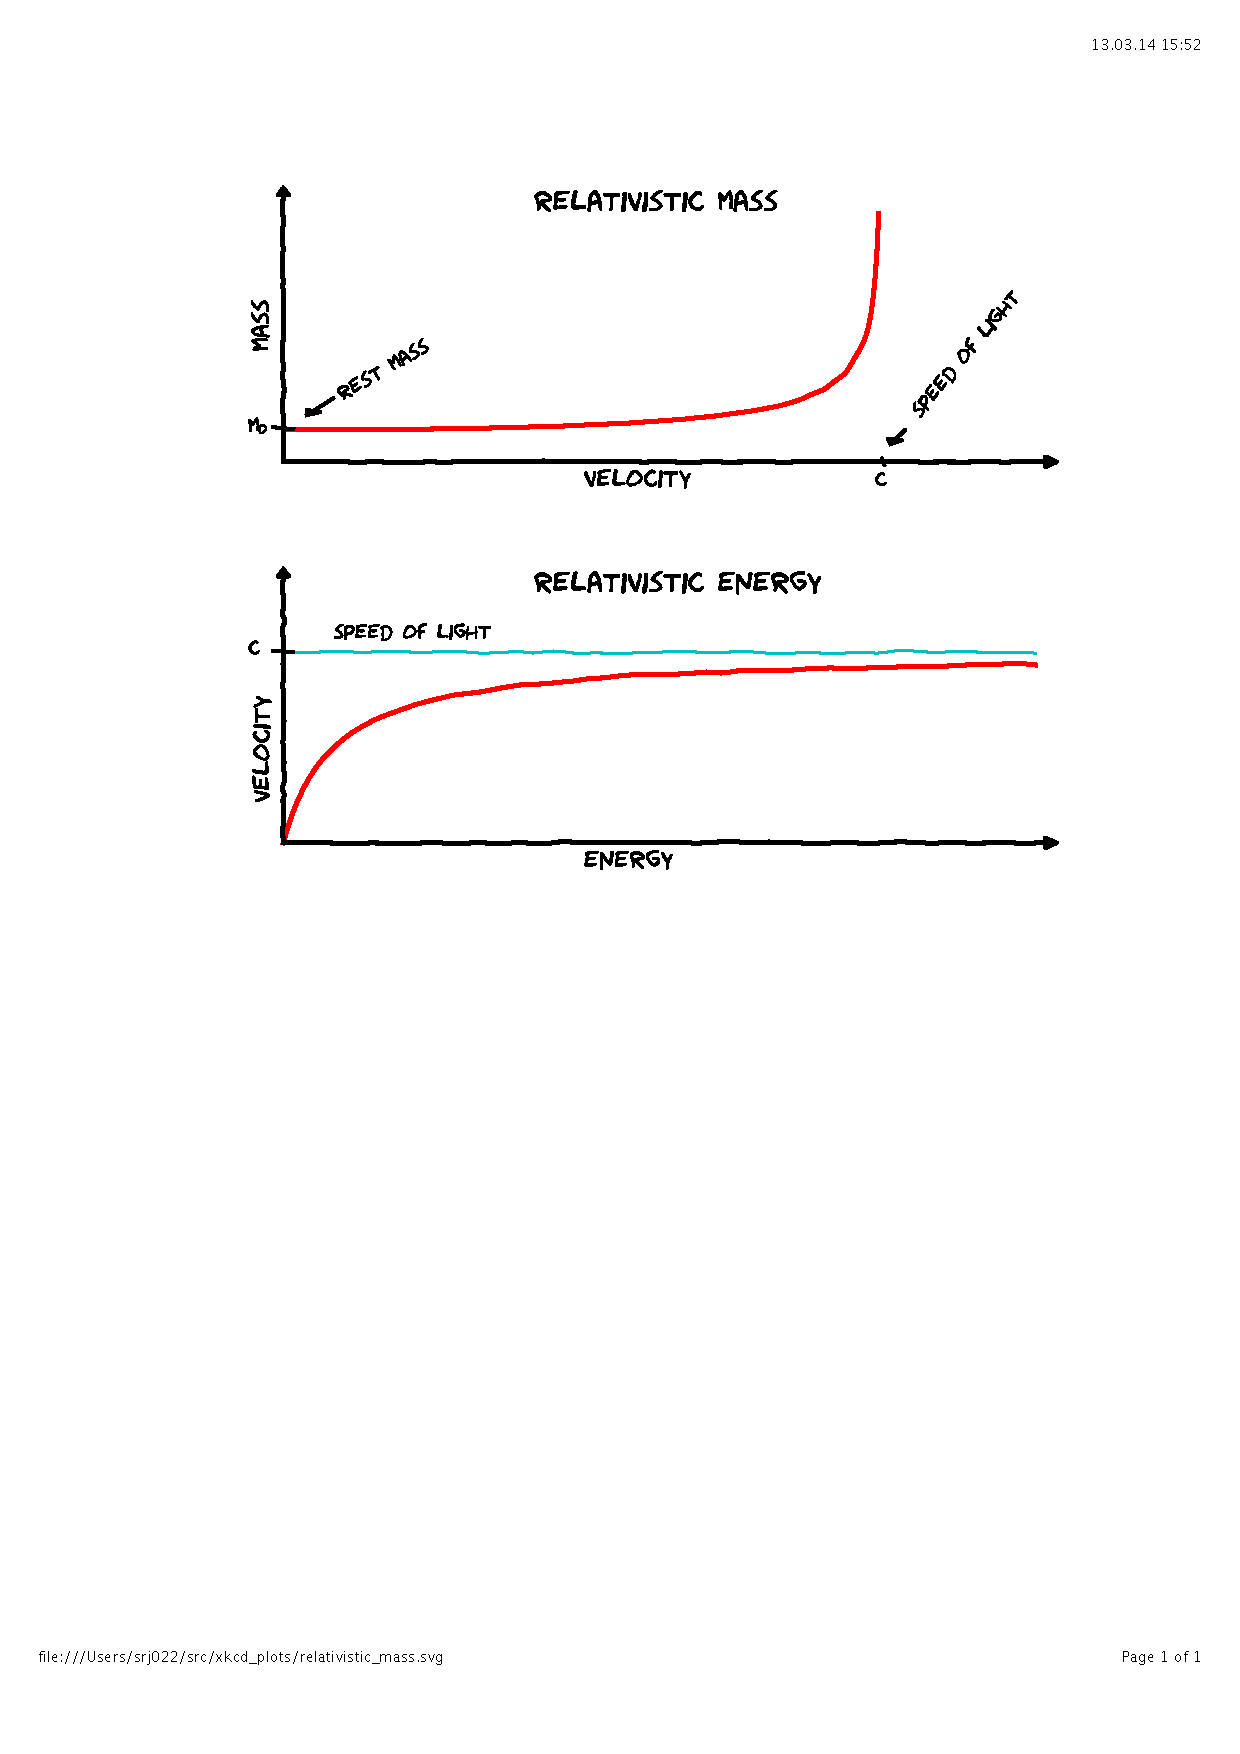
\includegraphics[viewport = 100 400 520 750, clip, scale=0.45]{figures/mass_and_energy.pdf}\\
    \end{column}
    \end{columns}
\end{frame}

\begin{frame}
    \frametitle{Relativistic effects in physics}
    \begin{columns}
    \begin{column}{.50\textwidth}
	\begin{equation}
	    \nonumber
	    E^2 = p^2c^2 + m^2c^4
	\end{equation}
	\ \\
	\ \\
	\begin{equation}
	    \nonumber
	    E = mc^2
	\end{equation}
    \end{column}
    \begin{column}{.50\textwidth}
	\centering
	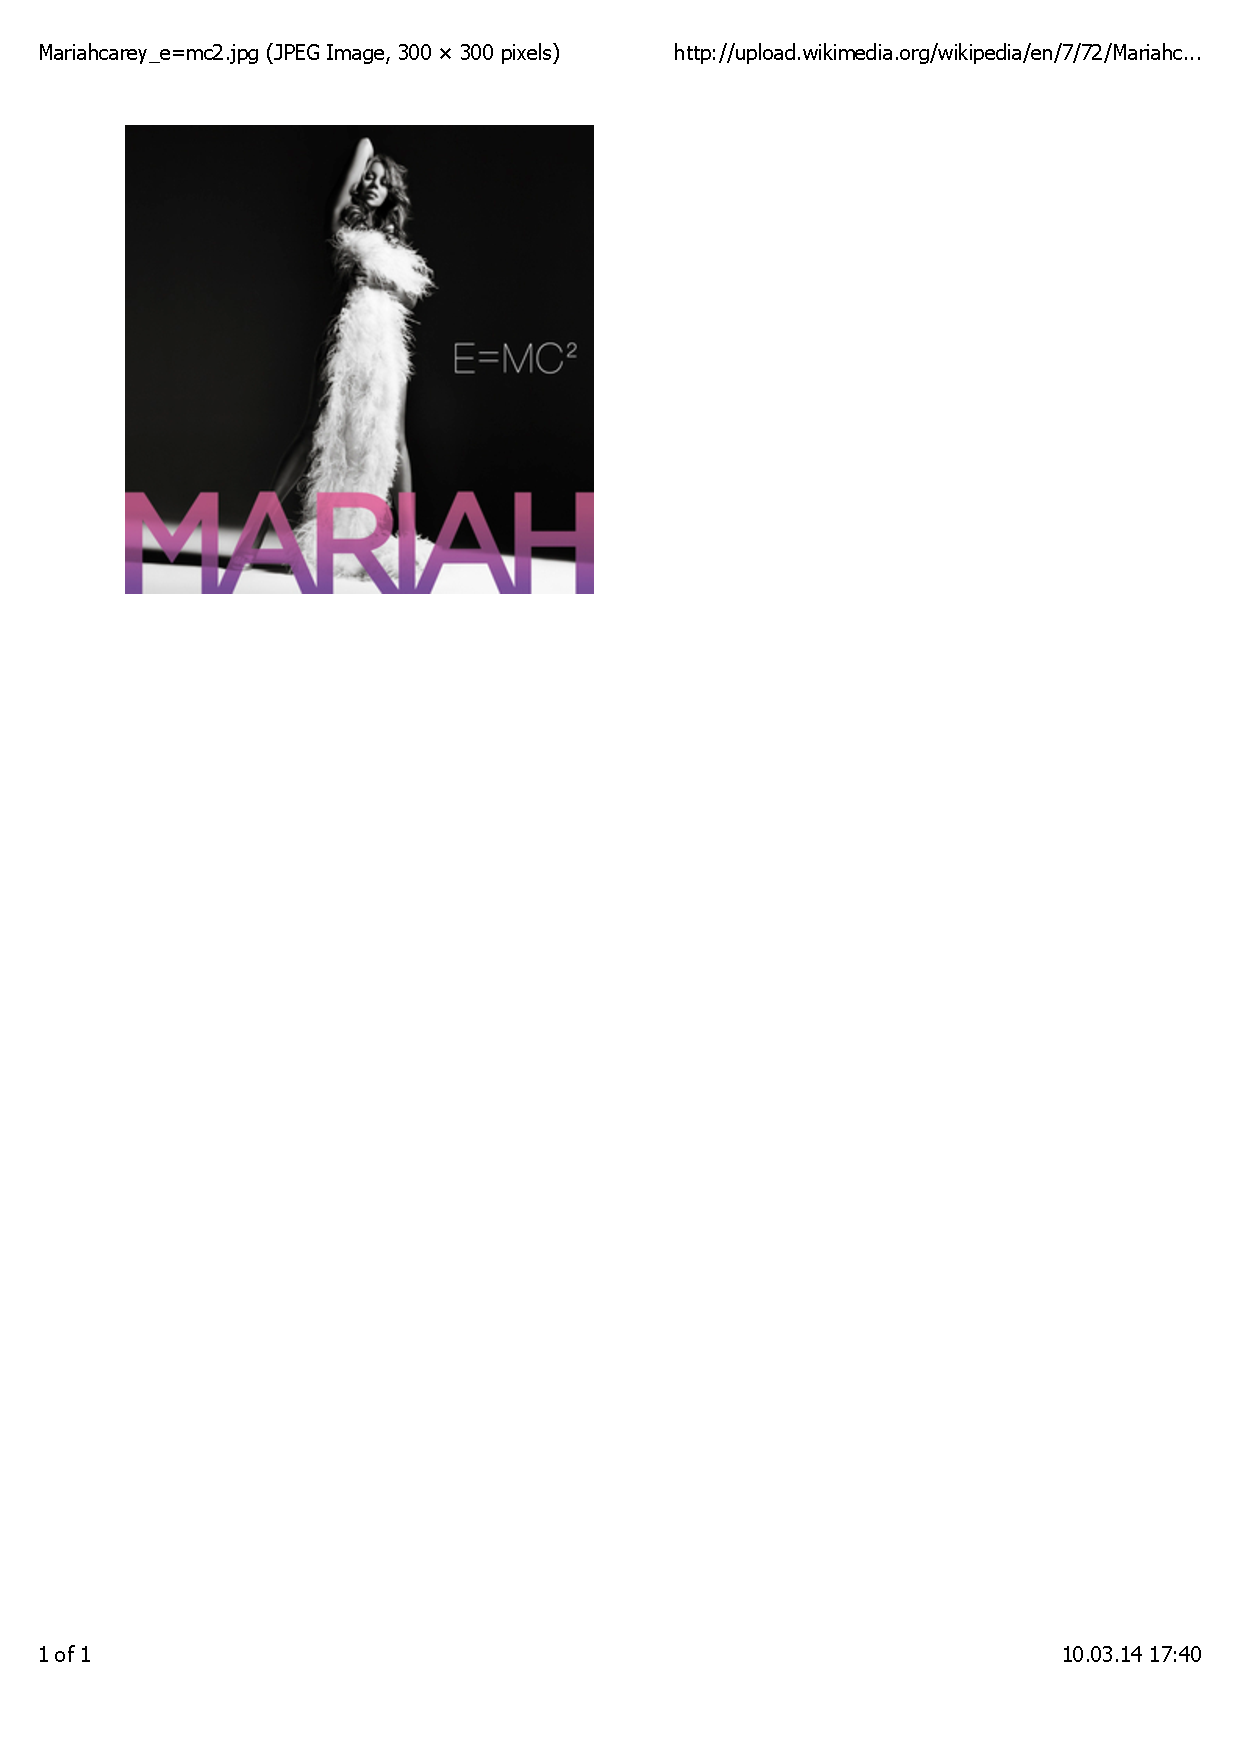
\includegraphics[viewport = 60 560 285 800, clip, scale=0.4]{figures/mariah.pdf}
    \end{column}
    \end{columns}
\end{frame}

\begin{frame}
    \frametitle{The Schr\"{o}dinger equation}
    \begin{columns}
    \begin{column}{.50\textwidth}
	\centering
	Time-independent equation
	\begin{equation}
	\nonumber
	    \hat{H} \psi = E \psi
	\end{equation}
	\ \\
	\begin{equation}
	    \nonumber
	    \hat{H} \psi = \left[\frac{\boldsymbol{p}^2}{2m} - eV \right] \psi
	\end{equation}
    \ \\
    \end{column}
    \begin{column}{.50\textwidth}
	\centering
	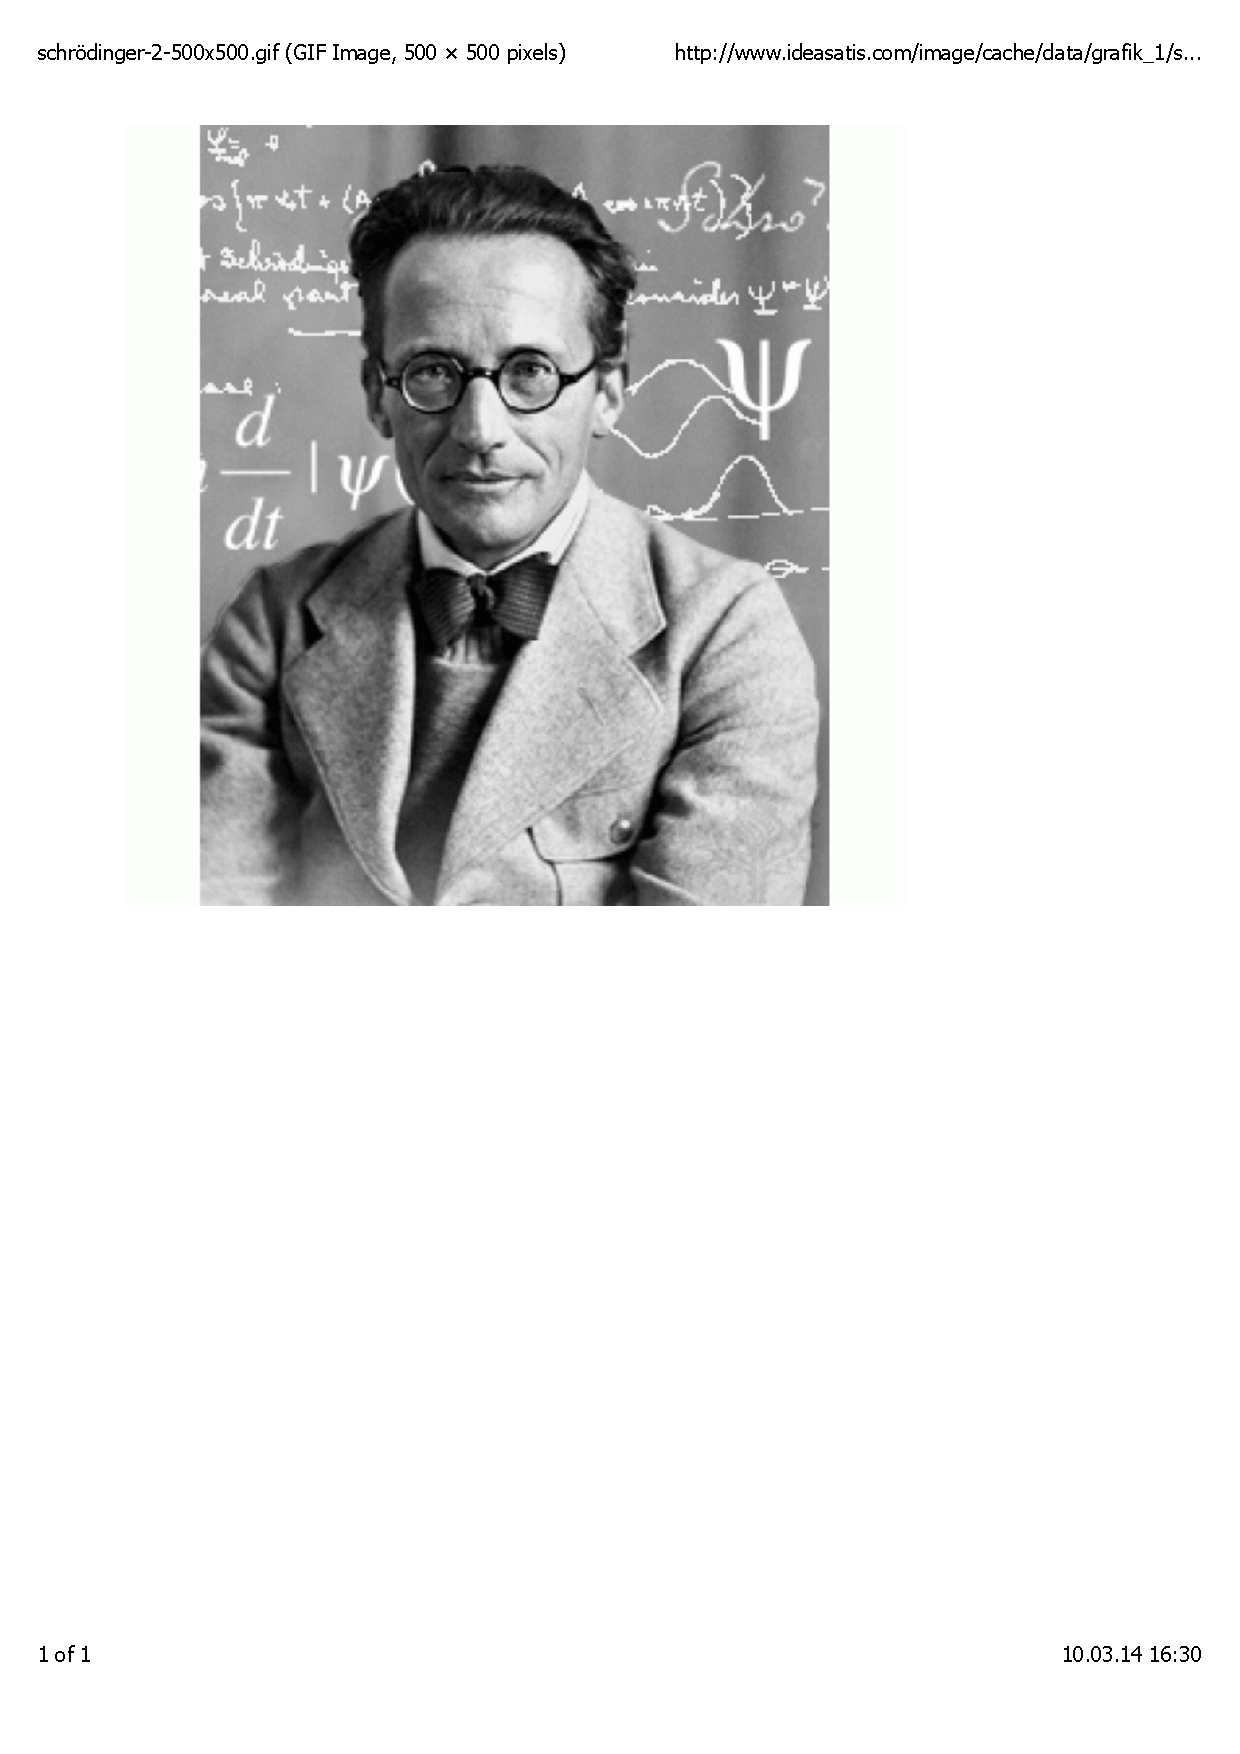
\includegraphics[viewport = 90 405 400 795, clip, scale=0.23]{figures/schrodinger.pdf}
    \end{column}
    \end{columns}
    \ \\
    \ \\
    \begin{equation}
	\nonumber
        g(\boldsymbol{r}_1,\boldsymbol{r}_2) = \frac{1}{r_{12}}
    \end{equation}
\end{frame}

\begin{frame}
    \frametitle{The Dirac equation}
    \begin{columns}
    \begin{column}{.60\textwidth}
	\centering
	Time-independent equation
	\begin{equation}
	    \nonumber
	    \hat{H} \psi = E \psi
	\end{equation}
	\ \\
	\ \\
	Four-component Hamiltonian
	\begin{equation}
	    \nonumber
	    \hat{H} = 
	    \begin{bmatrix}
		(mc^2 - eV) & c\boldsymbol{\sigma}\cdot\boldsymbol{p}\\
		c\boldsymbol{\sigma}\cdot\boldsymbol{p} & -(mc^2 - eV)\\
	    \end{bmatrix}
	\end{equation}
	\ \\
	\ \\
	\ \\
	Four-component wave function
	\begin{equation}
	    \nonumber
	    \psi = 
	    \begin{bmatrix}
		\psi_\alpha^L,
		\psi_\beta^L,
		\psi_\alpha^S, 
		\psi_\beta^S 
	    \end{bmatrix}
	\end{equation}
    \end{column}
    \begin{column}{.40\textwidth}
	\centering
	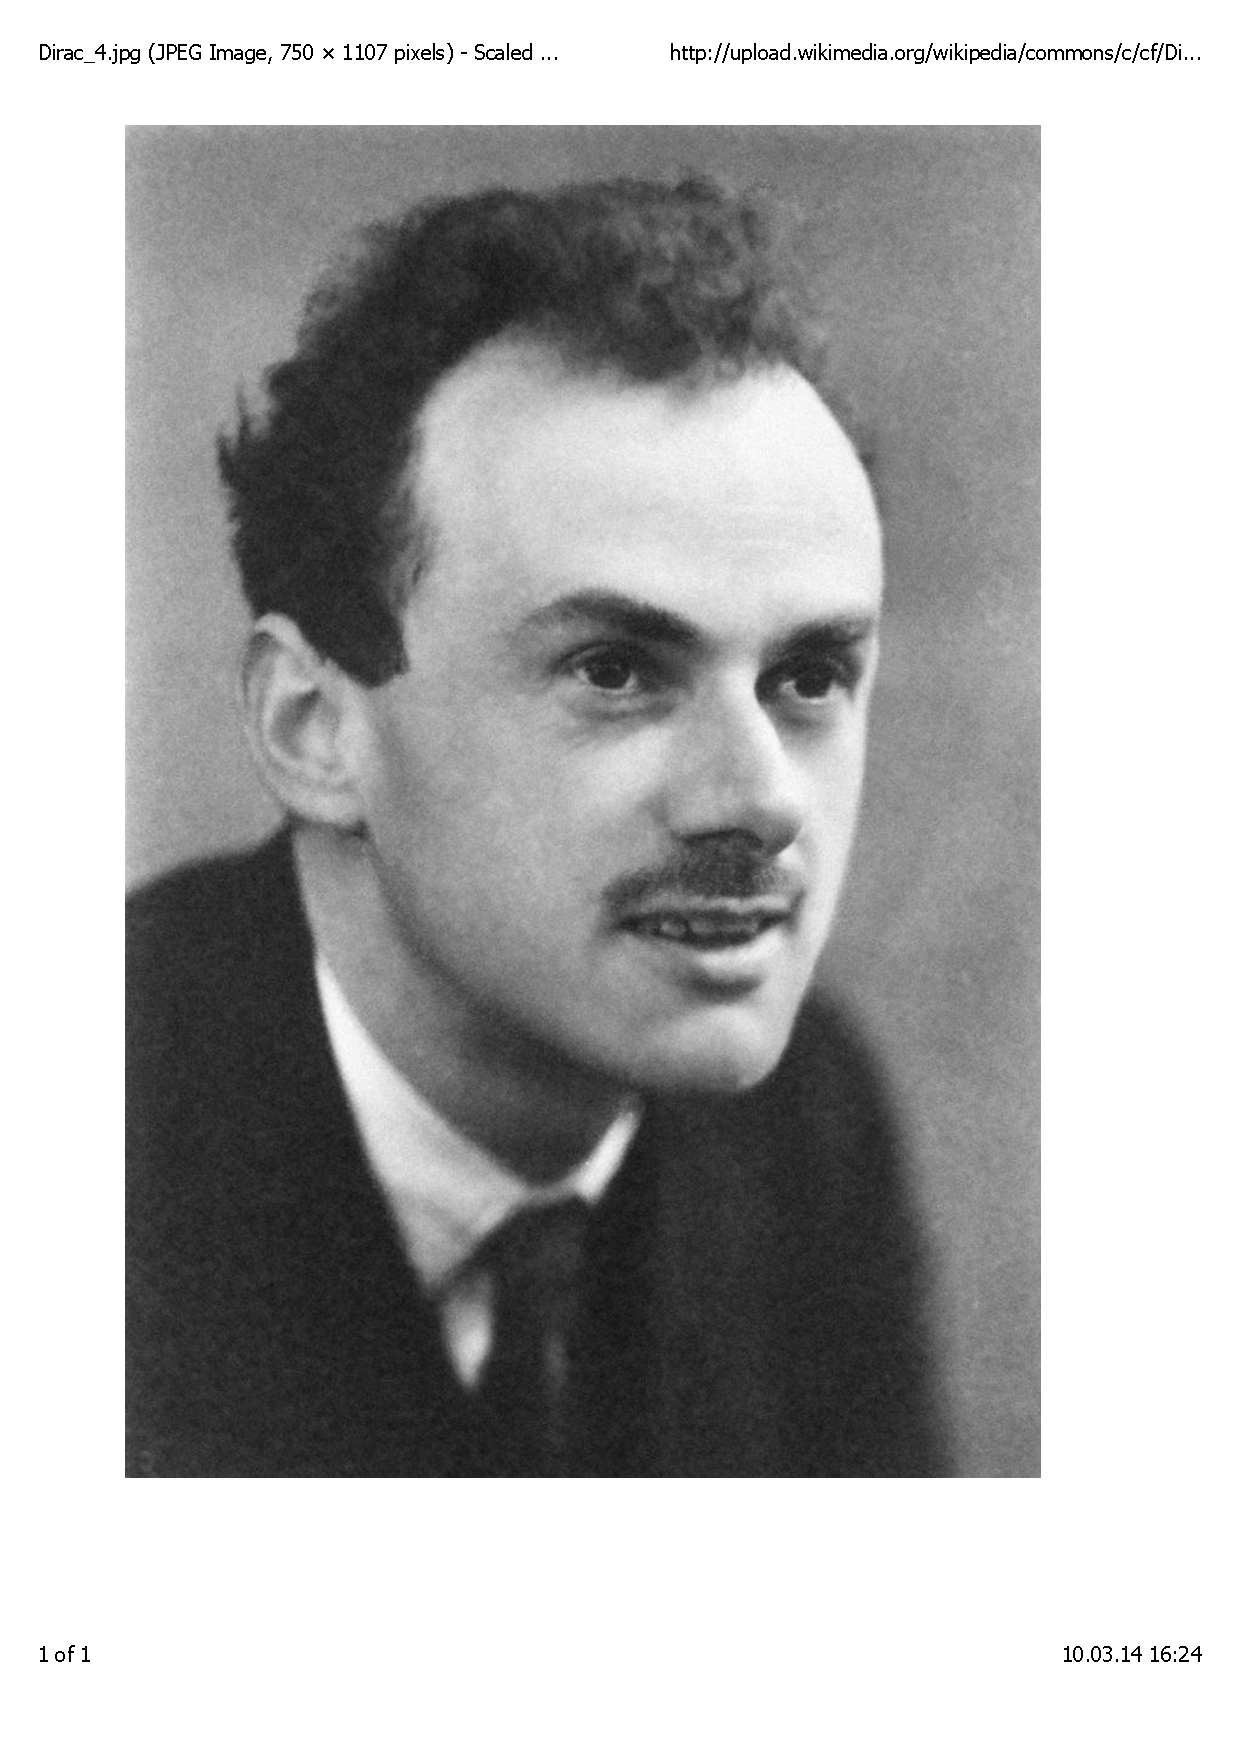
\includegraphics[viewport = 50 200 500 800, clip, scale=0.15]{figures/dirac.pdf}
    \end{column}
    \end{columns}
    \ \\
    \ \\
    \ \\
    \pause
    \centering
    Two-electron interaction
    \begin{equation}
        \nonumber
        g(\boldsymbol{r}_1,\boldsymbol{r}_2) = 
        \frac{1}{r_{12}} - \frac{c\boldsymbol{\alpha}_1\cdot c\boldsymbol{\alpha}_2}{c^2r_{12}} -
        \frac{(c\boldsymbol{\alpha}_1\cdot \boldsymbol{r}_{12})(c\boldsymbol{\alpha}_2\cdot \boldsymbol{r}_{12})}{c^2r_{12}^3}
        + \cdots
    \end{equation}
\end{frame}

\begin{frame}
    \frametitle{Relativistic free particle}
    \begin{columns}
    \begin{column}{.40\textwidth}
	\centering
	Free particle energy
        \begin{equation}
	   \nonumber
	   E = \pm \sqrt{p^2c^2+m^2c^4}
	\end{equation}
	\ \\
	\ \\
	\ \\
	\begin{itemize}
	    \item Negative energy states
	    \item Dirac sea
	    \item Electron-positron pair
	\end{itemize}
    \end{column}
    \begin{column}{.60\textwidth}
	\centering
	\only<1>{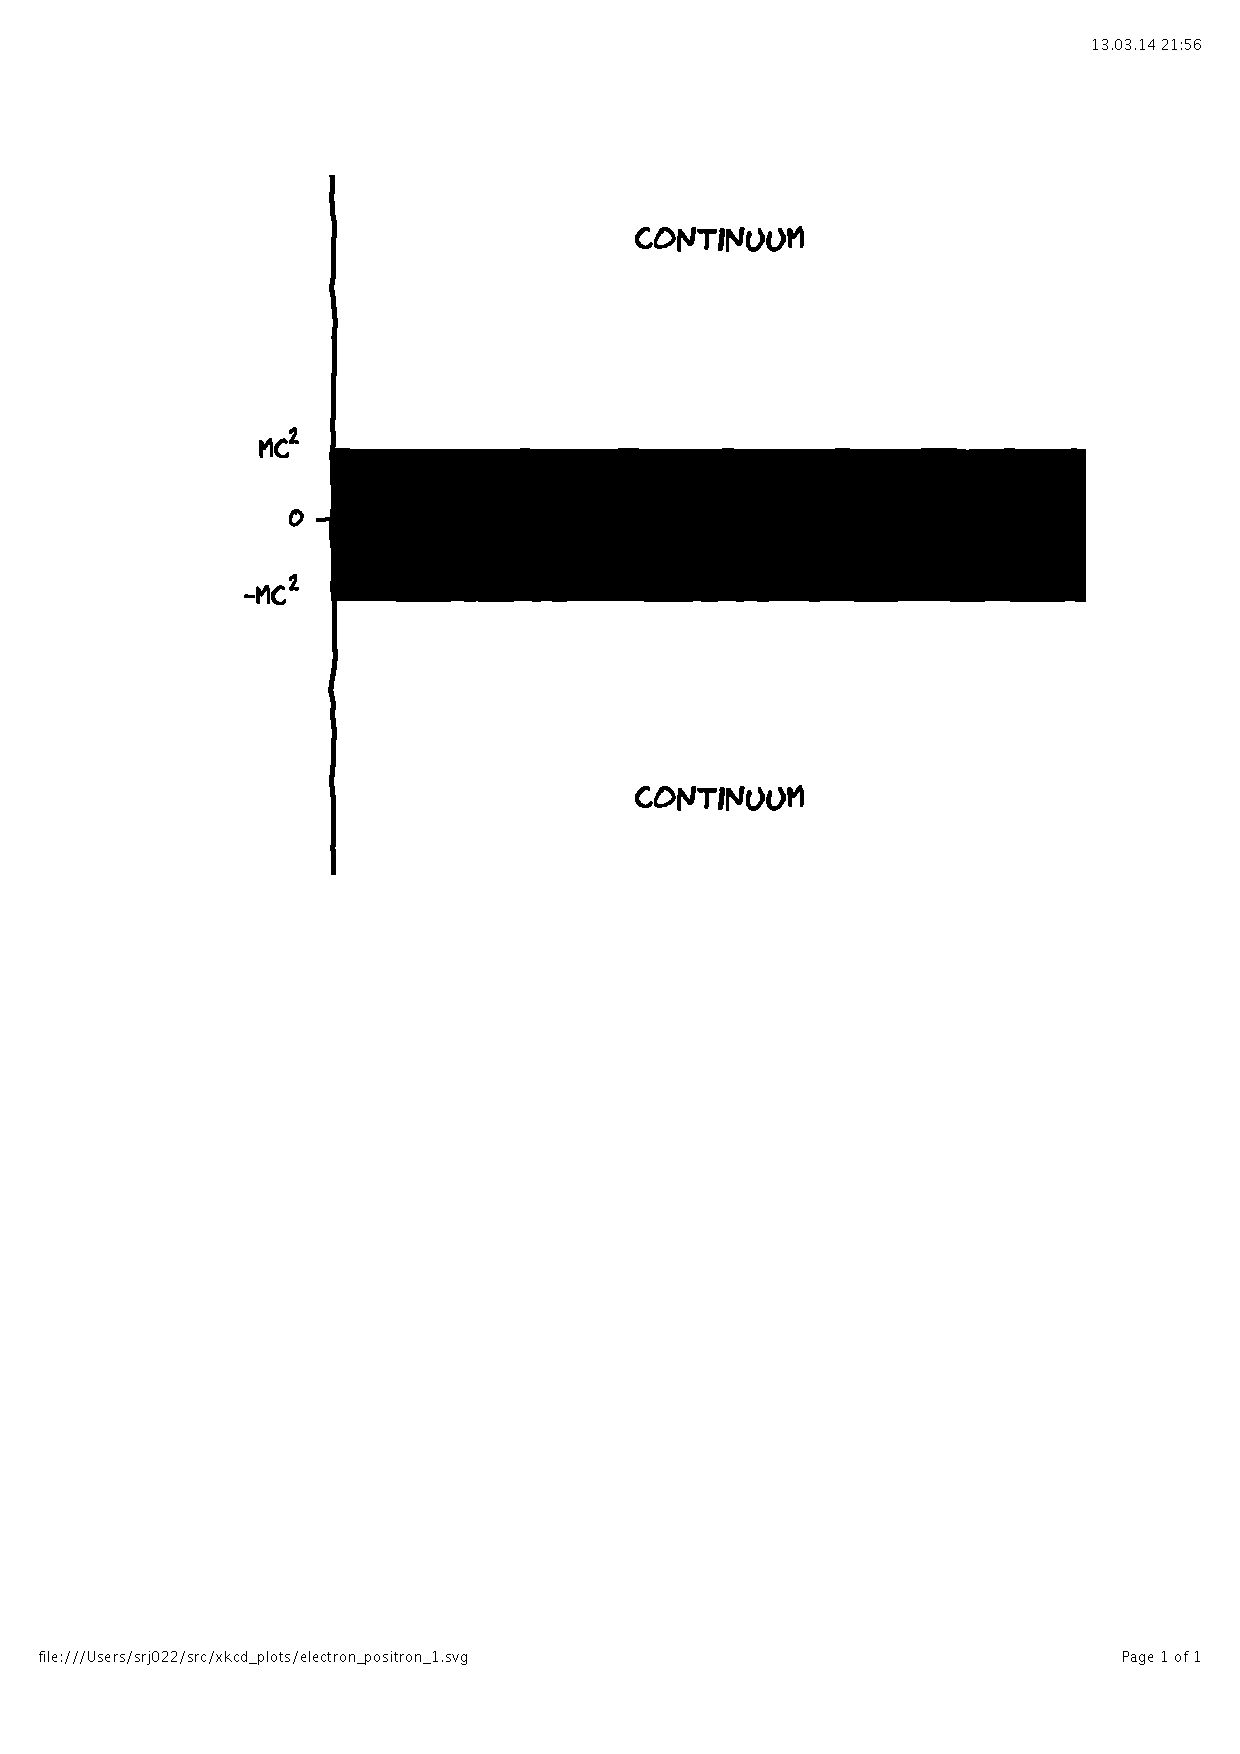
\includegraphics[viewport = 100 420 520 750, clip, scale=0.4]{figures/electron_positron_1.pdf}}
	\only<2>{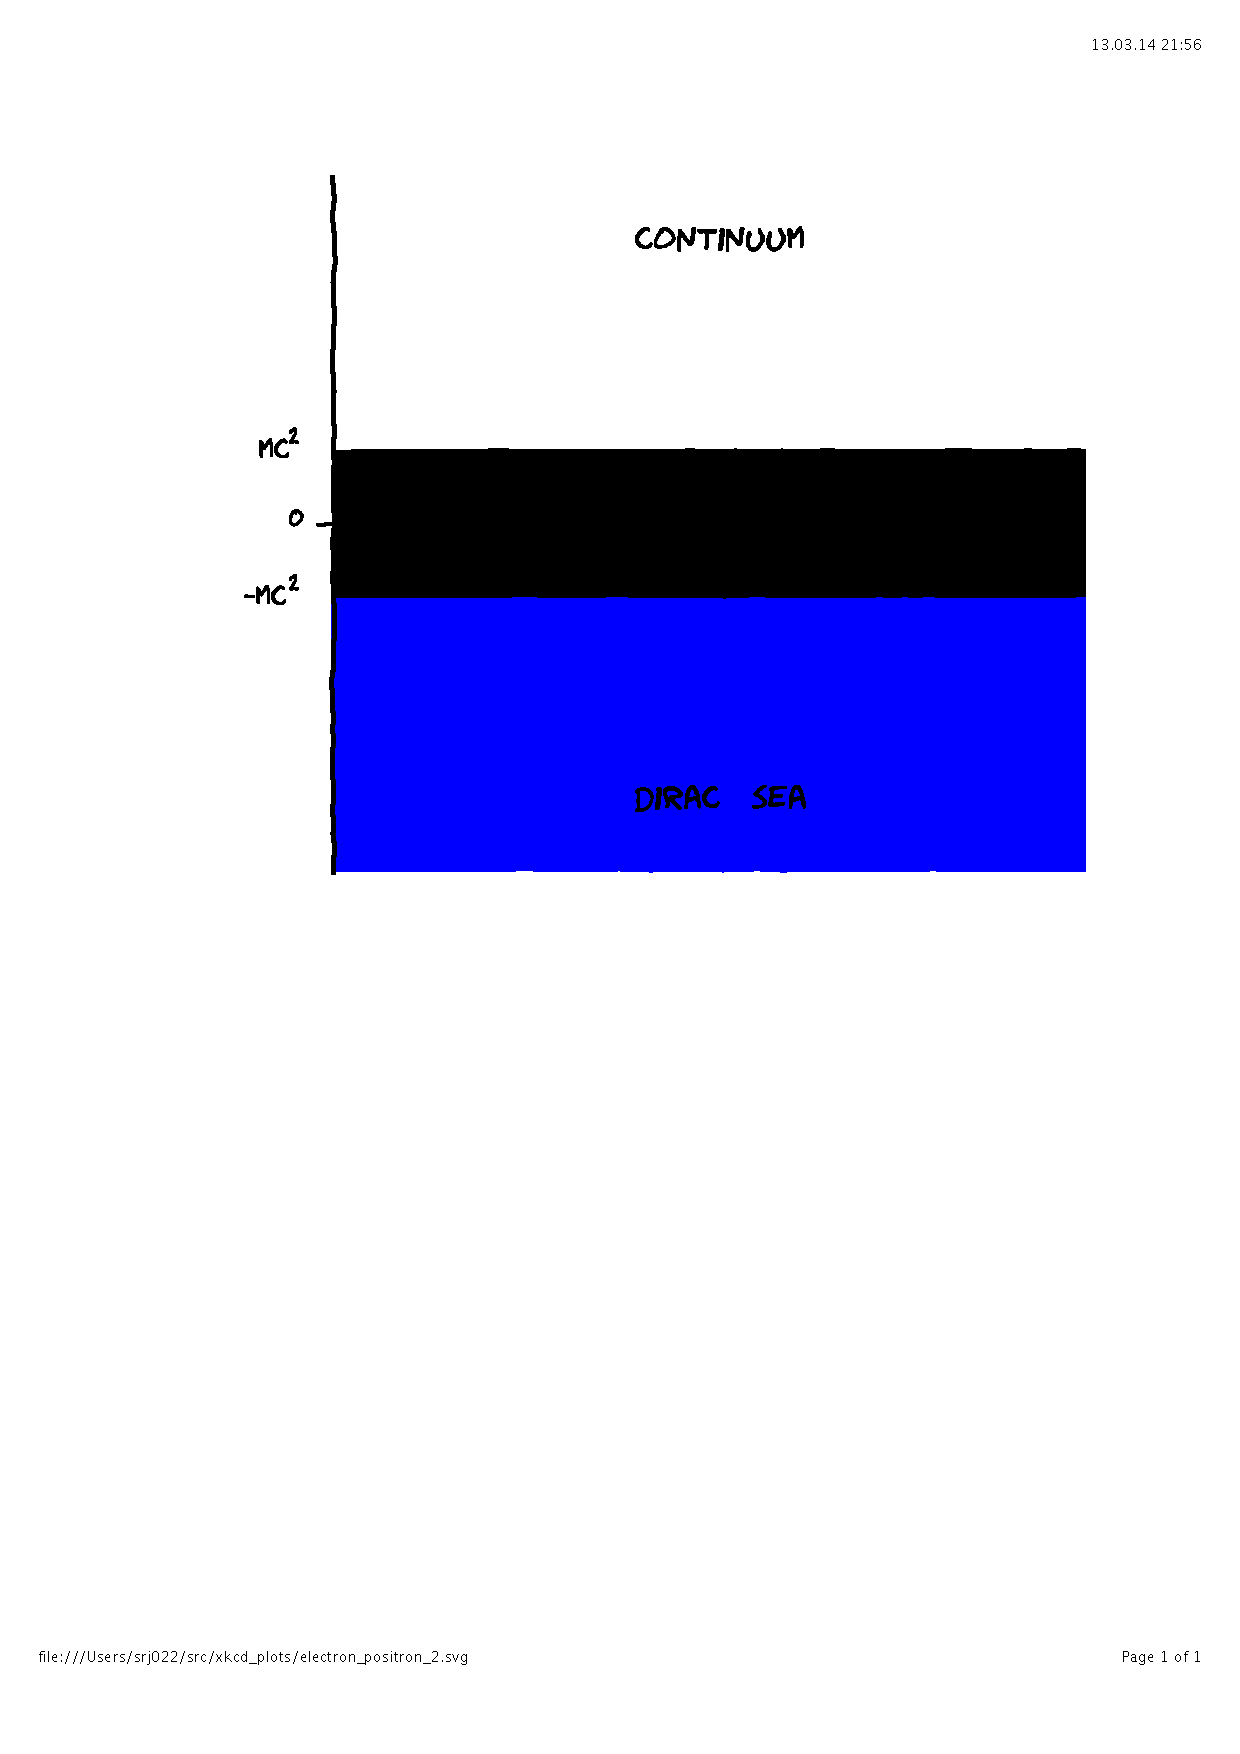
\includegraphics[viewport = 100 420 520 750, clip, scale=0.4]{figures/electron_positron_2.pdf}}
	\only<3>{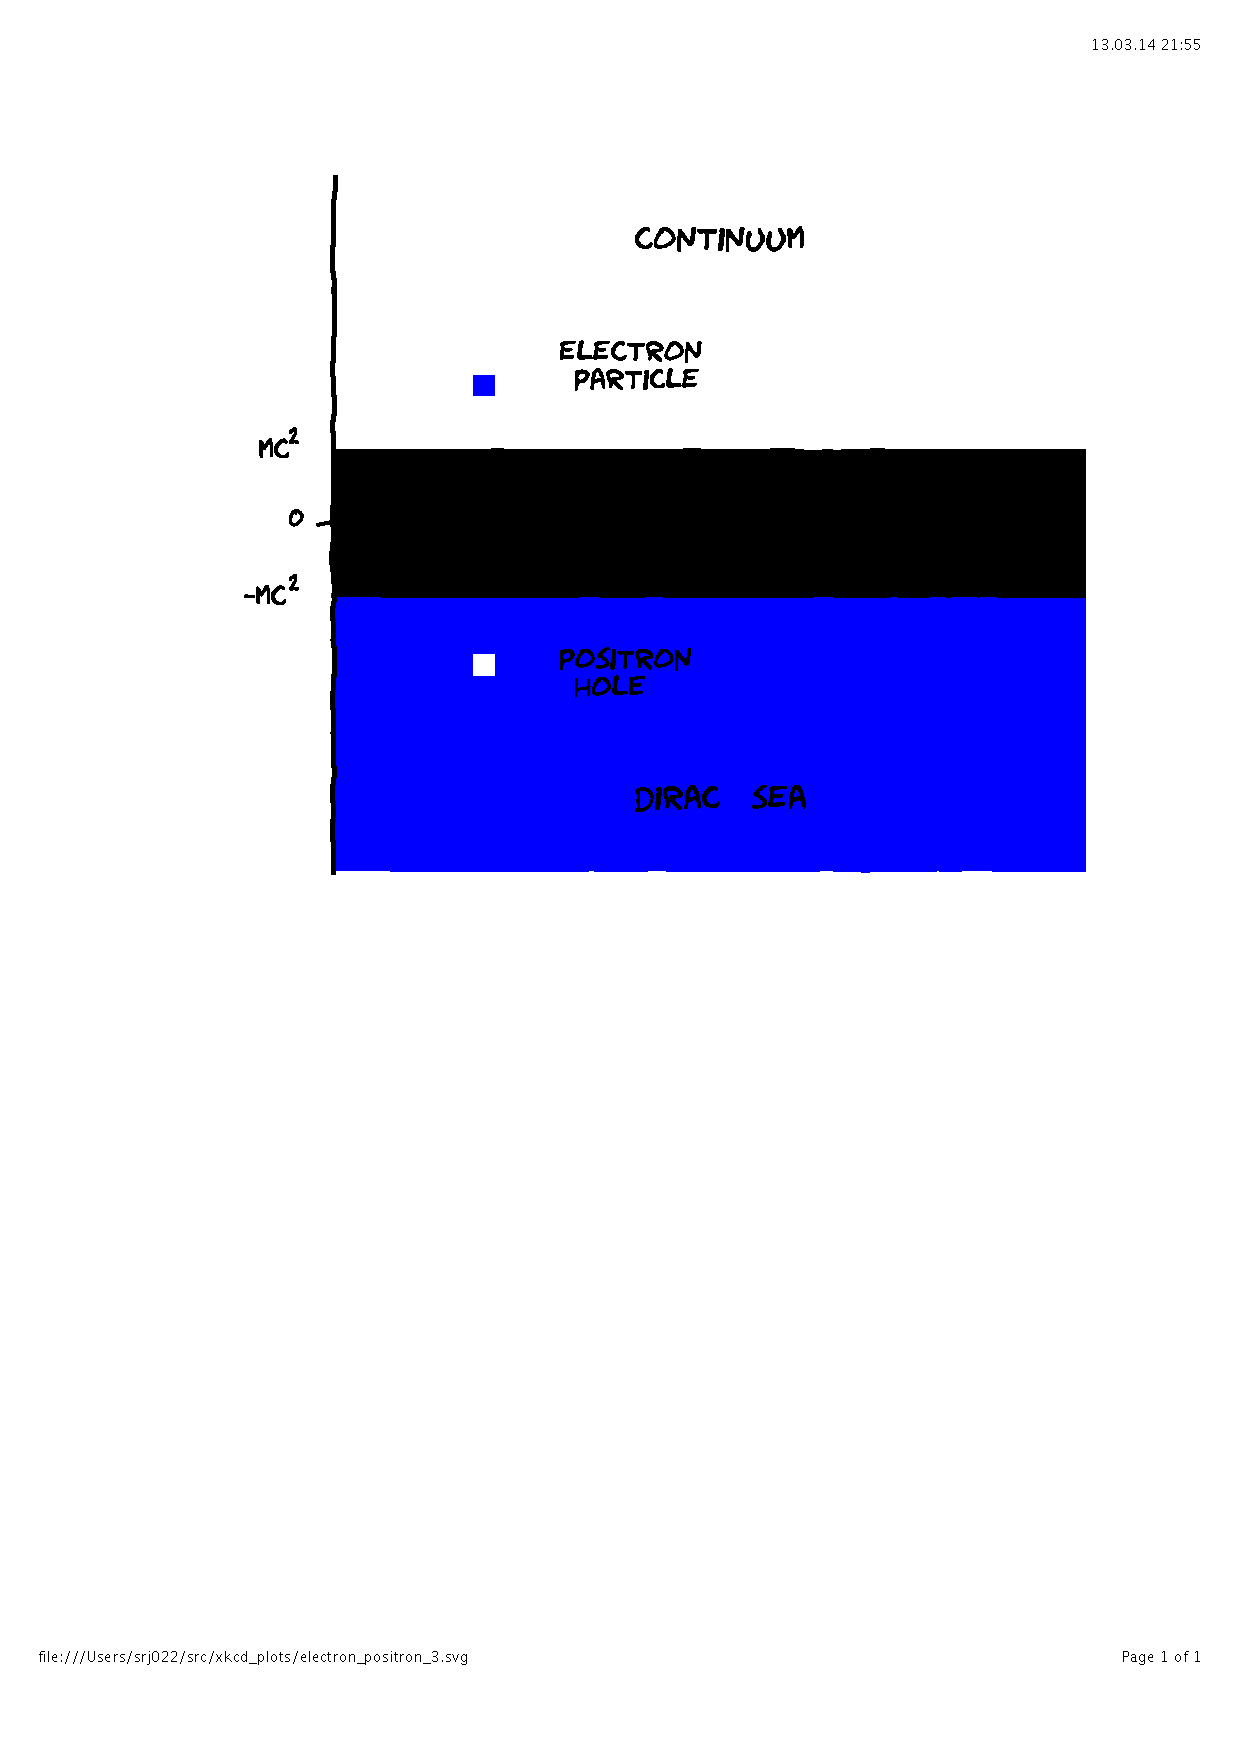
\includegraphics[viewport = 100 420 520 750, clip, scale=0.4]{figures/electron_positron_3.pdf}}
    \end{column}
    \end{columns}
\end{frame}

\begin{frame}
    \frametitle{Relativistic atomic structure}
    \begin{columns}
    \begin{column}{.40\textwidth}
	\centering
	Hydrogen atom energy
	\begin{equation}
	    \nonumber
	    E = -\frac{Z^2}{2n^2} + \frac{Z^4}{2n^2c^2}\left(\frac{3}{4}-\frac{n}{j+1/2}\right) + \cdots
	\end{equation}
	\begin{itemize}
	    \item Strong dependence on atomic number $Z$
	    \item Splitting of energy levels 
	    \item Orbital angular momentum $l$ and spin $m_s$ quantum numbers no longer appropriate
	    \item Total angular momentum $j$ is the proper quantum number
	\end{itemize}
    \end{column}
    \begin{column}{.40\textwidth}
    Plot of energy levels\\
    \end{column}
    \end{columns}
\end{frame}

\begin{frame}
    \frametitle{Approximate Hamiltonians}
    \begin{itemize}
    \item Pauli Hamiltoninan
    \begin{equation}
	\nonumber
	H^{pauli} = T + V + h^{mv} + h^{darwin} + h^{so} + \cdots
    \end{equation}
    \ \\
    \ \\
    \item Scalar relativistic effects
    \begin{align}
	\nonumber
	h^{mv} &= -\frac{p^4}{8m^3c^2}\\
	\nonumber
	h^{darwin} &= \frac{1}{8m^2c^2} \nabla^2V
    \end{align}
    \ \\
    \ \\
    \item Spin-orbit relativistic effects
    \ \\
    \begin{equation}
	\nonumber
	h^{so} = \frac{1}{4m^2c^2}\boldsymbol{\sigma}\cdot\left[\left(\nabla V\right)\times\boldsymbol{p}\right]
    \end{equation}
    \end{itemize}
\end{frame}

\begin{frame}
    \frametitle{Scalar relativistic effects}
    \begin{itemize}
	\item	Electron speed related to nuclear charge $Z$
		and principal quantum number $n$
		\begin{equation}
		    \nonumber
		    \frac{v_e}{c} \approx \frac{Z}{n\alpha},\qquad \alpha \approx 137
		\end{equation}
	\item	giving an \textbf{increase} in electron mass
		\begin{equation}
		    \nonumber
		    m_{rel} = \gamma m_e \approx \frac{m_e}{\sqrt{1-Z^2/(n\alpha)^2}}
		\end{equation}
	\item	\textbf{contraction} of the Bohr radius
		\begin{equation}
		    \nonumber
		    a_{rel} = \frac{a_0}{\gamma} \approx a_0\sqrt{1-Z^2/(n\alpha)^2}
		\end{equation}
	\item	and the \textbf{mass-velocity} energy correction
		\begin{equation}
		    \nonumber
		    h^{mv} = -\frac{p^4}{8m^3c^2}
		\end{equation}
	\item	Relativity leads to \textbf{orbital contraction} and a \textbf{lowering} of the energy, 
		and the effect is greater with higher nuclear charge and lower principal quantum number
	\end{itemize}
\end{frame}

\begin{frame}
    \frametitle{Scalar relativistic effects}
    \ \\
    \centering
    The Darwin energy correction
    \begin{equation}
	\nonumber
	h^{darwin} = \frac{1}{8m^2c^2} \nabla^2 V
    \end{equation}
    \ \\
    \begin{columns}
    \begin{column}{.40\textwidth}
    \ \\
    \ \\
    \begin{itemize}
	\item Originates from ''zitterbewegung''\\
    \ \\
	\item Energy from oscillatory motion of the electron\\
    \ \\
	\item Contiuous creation and annihilation of electron-positron pairs
    \end{itemize}
    \ \\
    \end{column}
    \begin{column}{.60\textwidth}
	\centering
	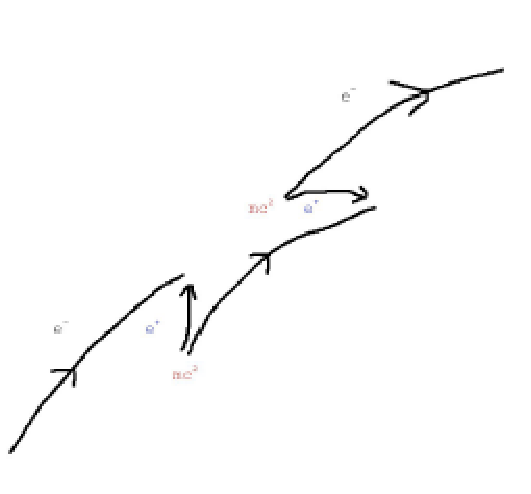
\includegraphics[viewport = 0 0 300 300, clip, scale=0.4]{figures/zitterbewegung.pdf}
    \end{column}
    \end{columns}
\end{frame}

\begin{frame}
    \frametitle{Spin-orbit effects}
    \begin{equation}
	\nonumber
	h^{so} = \frac{1}{4m^2c^2}\boldsymbol{\sigma}\cdot\left[\left(\nabla V\right)\times\boldsymbol{p}\right]
    \end{equation}
\end{frame}

\begin{frame}
    \frametitle{Relativistic computational chemistry}
    \begin{columns}
    \begin{column}{.40\textwidth}
    \ \\
    \ \\
    \begin{itemize}
	\item Dirac
	\item ReSpect
	\item Solvent effect through PCMSolver Dirac
    \end{itemize}
    \ \\
    \end{column}
    \begin{column}{.60\textwidth}
	\centering
	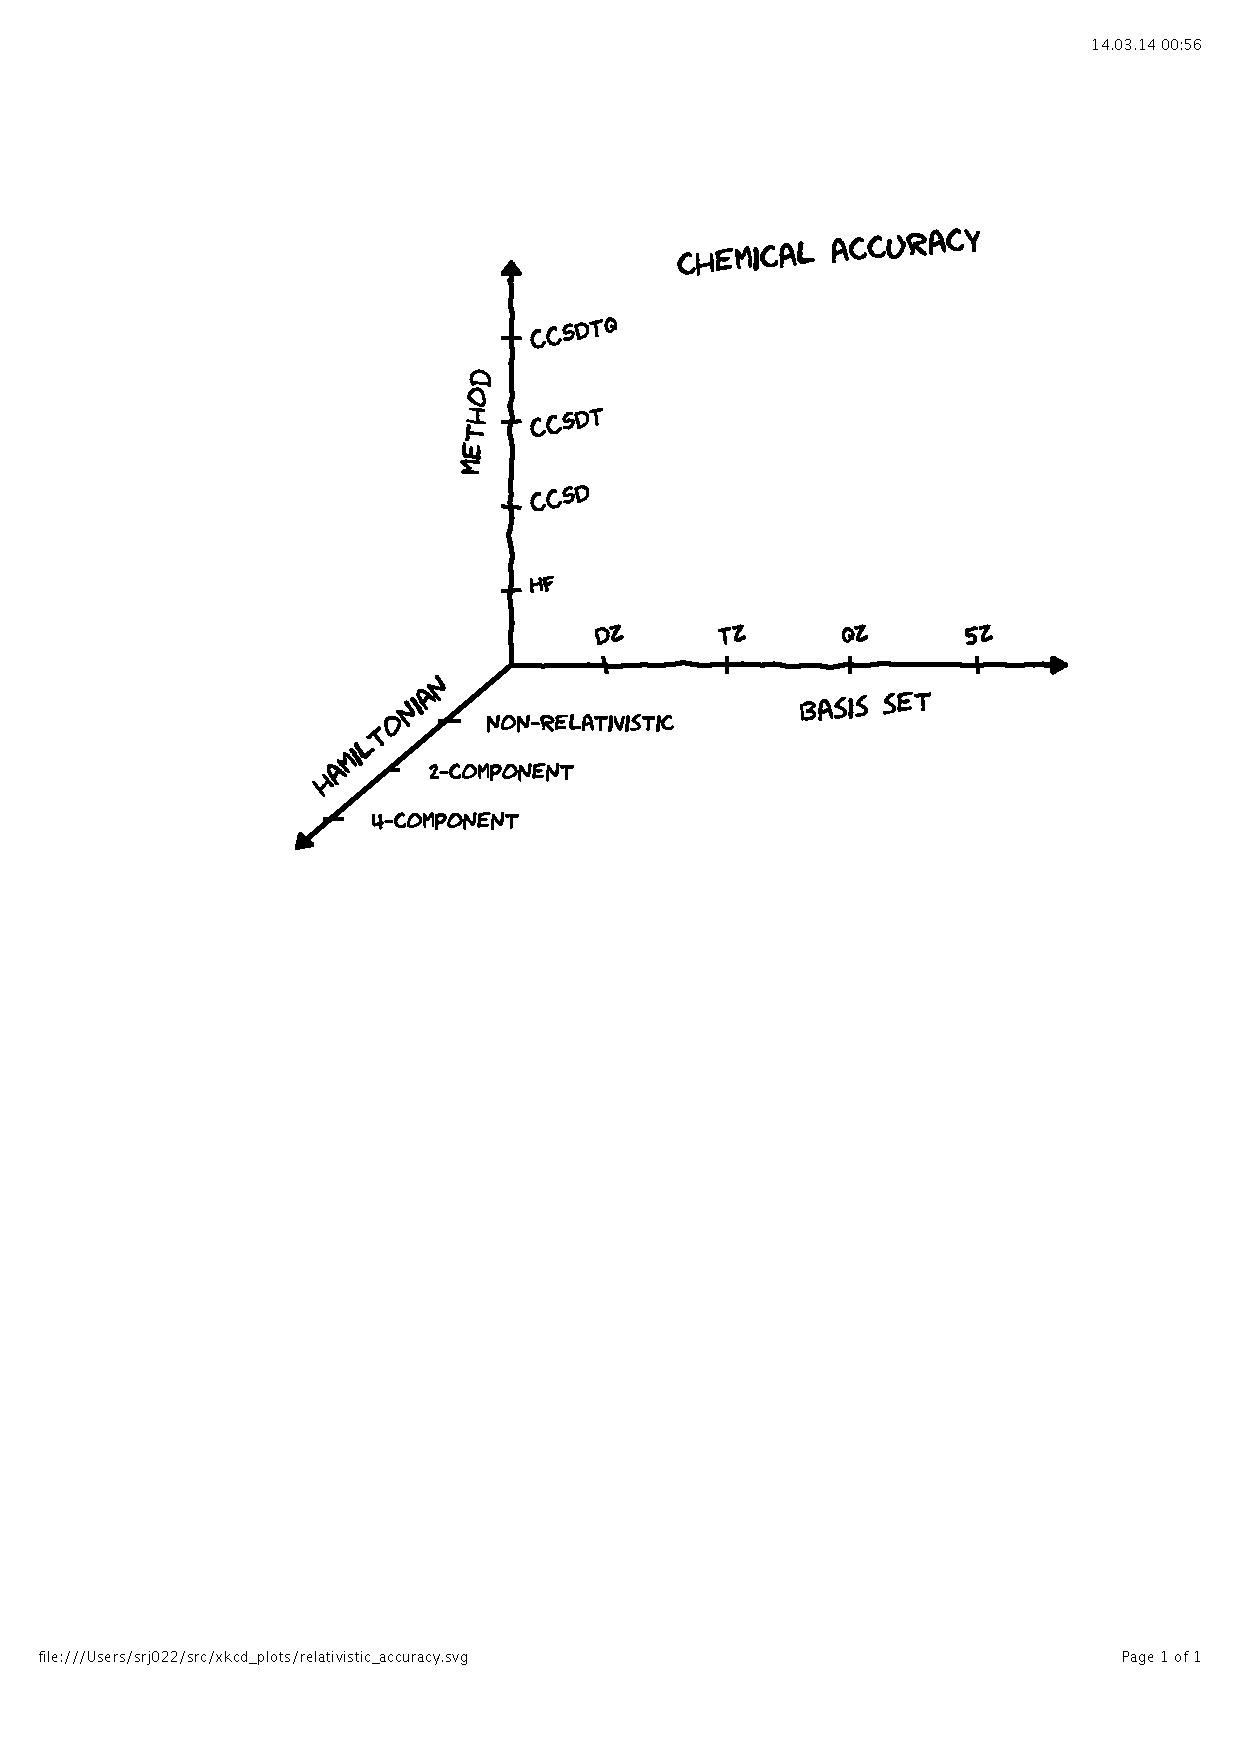
\includegraphics[viewport = 100 400 600 800, clip, scale=0.3]{figures/relativistic_accuracy.pdf}
    \end{column}
    \end{columns}
\end{frame}

\begin{frame}
    \frametitle{The periodic table}
    \begin{columns}
    \begin{column}{.40\textwidth}
	Lantanide contraction\\
	Pyykko's PT
    \end{column}
    \begin{column}{.60\textwidth}
	\centering
	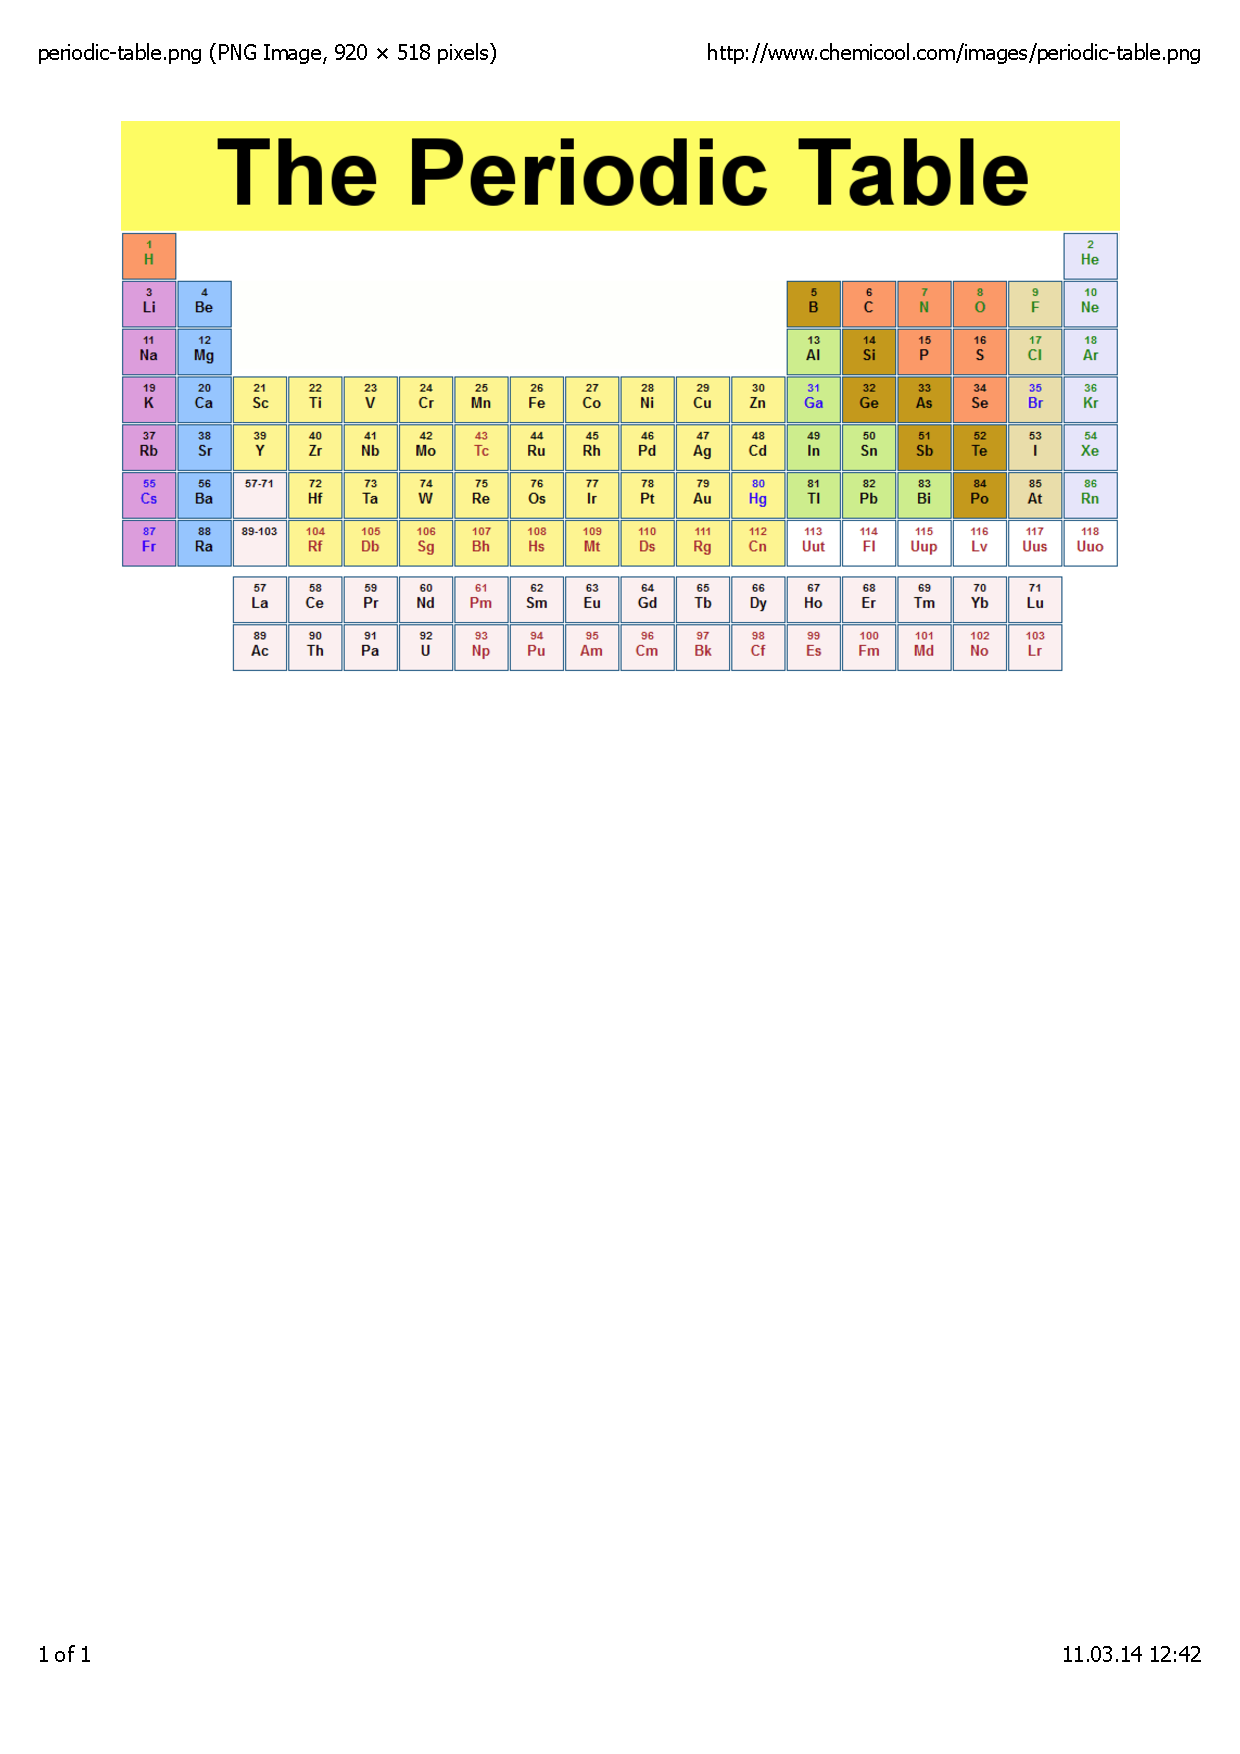
\includegraphics[viewport = 0 500 550 800, clip, scale=0.3]{figures/periodic_table.pdf}
    \end{column}
    \end{columns}
\end{frame}

\begin{frame}
    \frametitle{The color of gold}
    \begin{columns}
    \begin{column}{.50\textwidth}
	\ \\
    \end{column}
    \begin{column}{.50\textwidth}
	\centering
	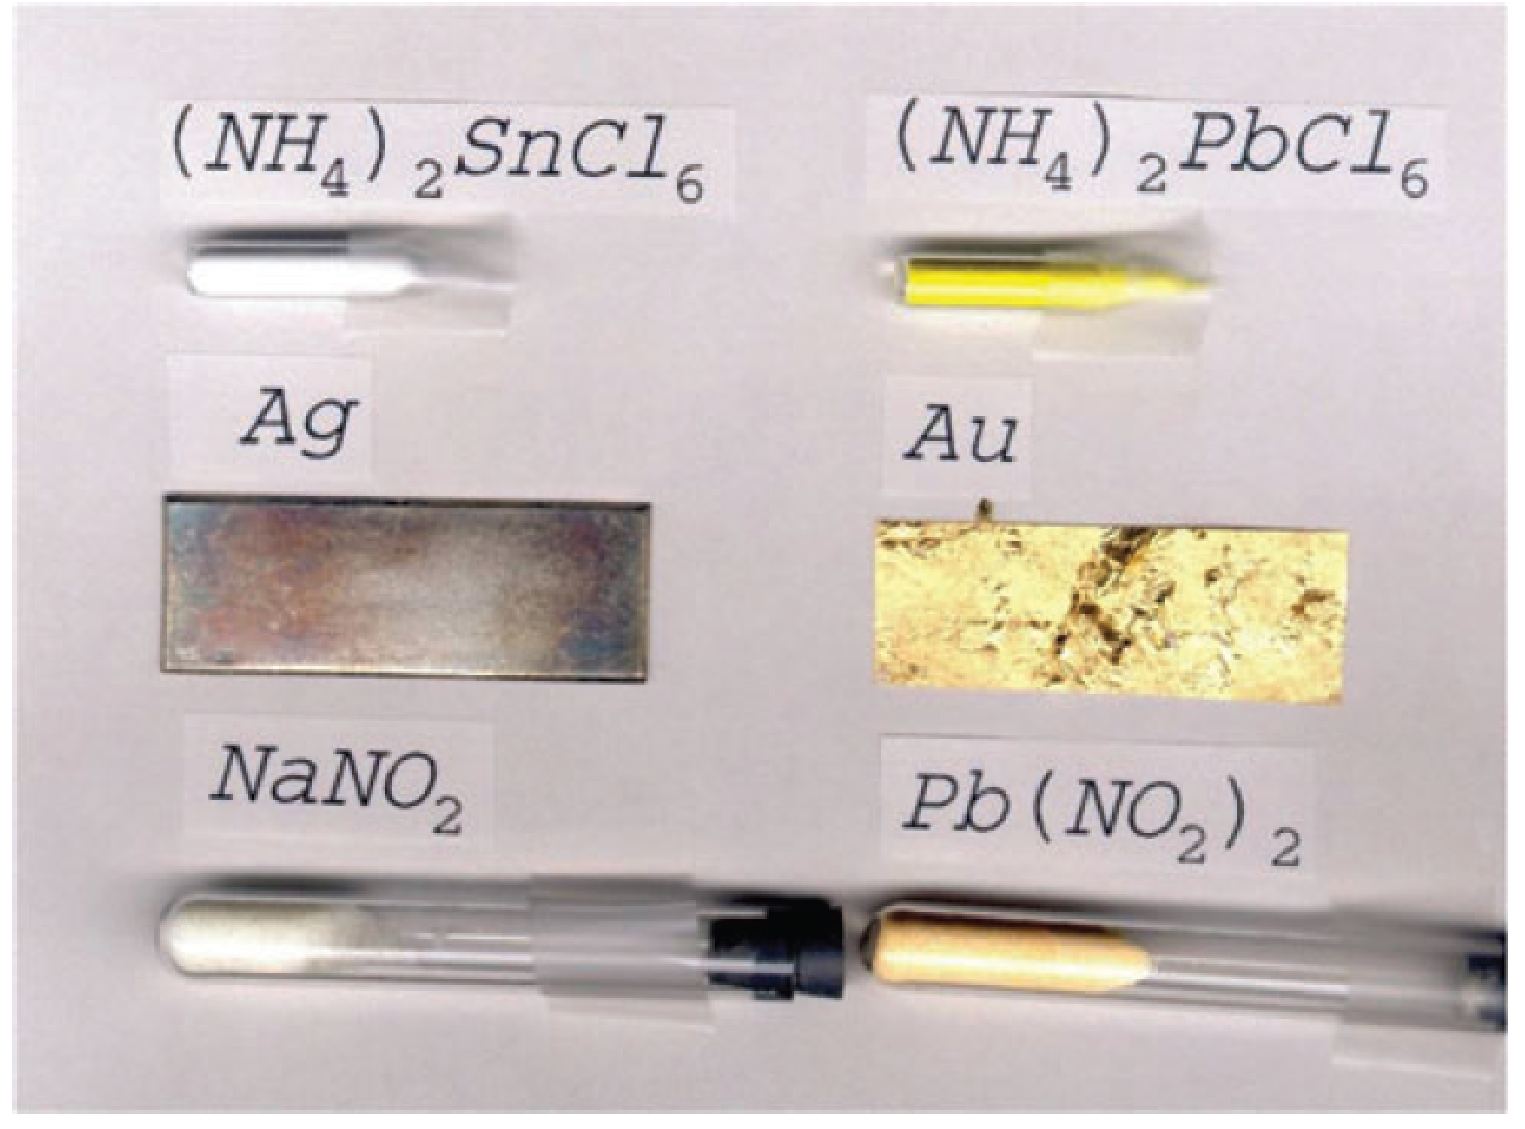
\includegraphics[viewport = 0 0 800 550, clip, scale=0.15]{figures/gold.pdf}
    \end{column}
    \end{columns}
\end{frame}

\begin{frame}
    \frametitle{Lead-acid battery}
    \begin{columns}
    \begin{column}{.50\textwidth}
	\ \\
    \end{column}
    \begin{column}{.50\textwidth}
	\centering
	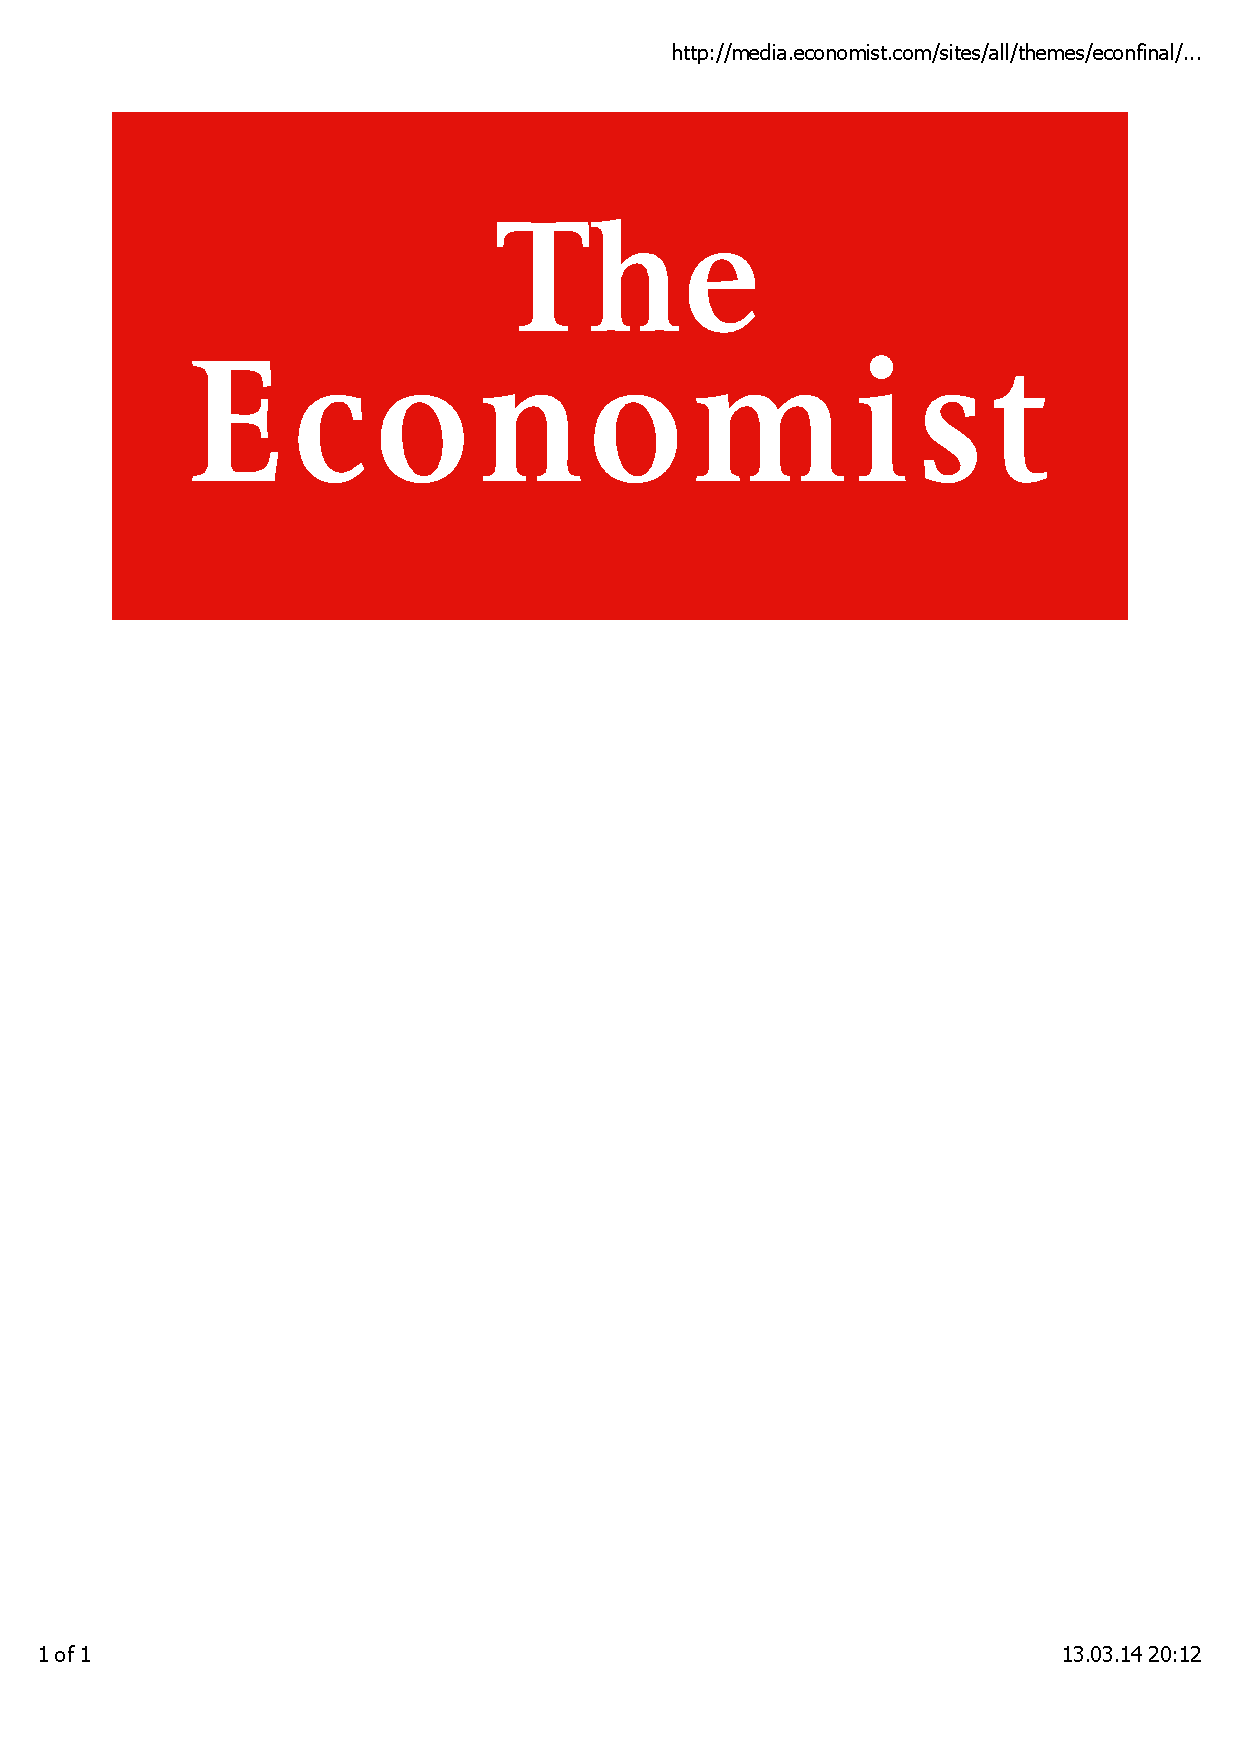
\includegraphics[viewport = 0 550 600 800, clip, scale=0.1]{figures/economist_logo.pdf}\\
	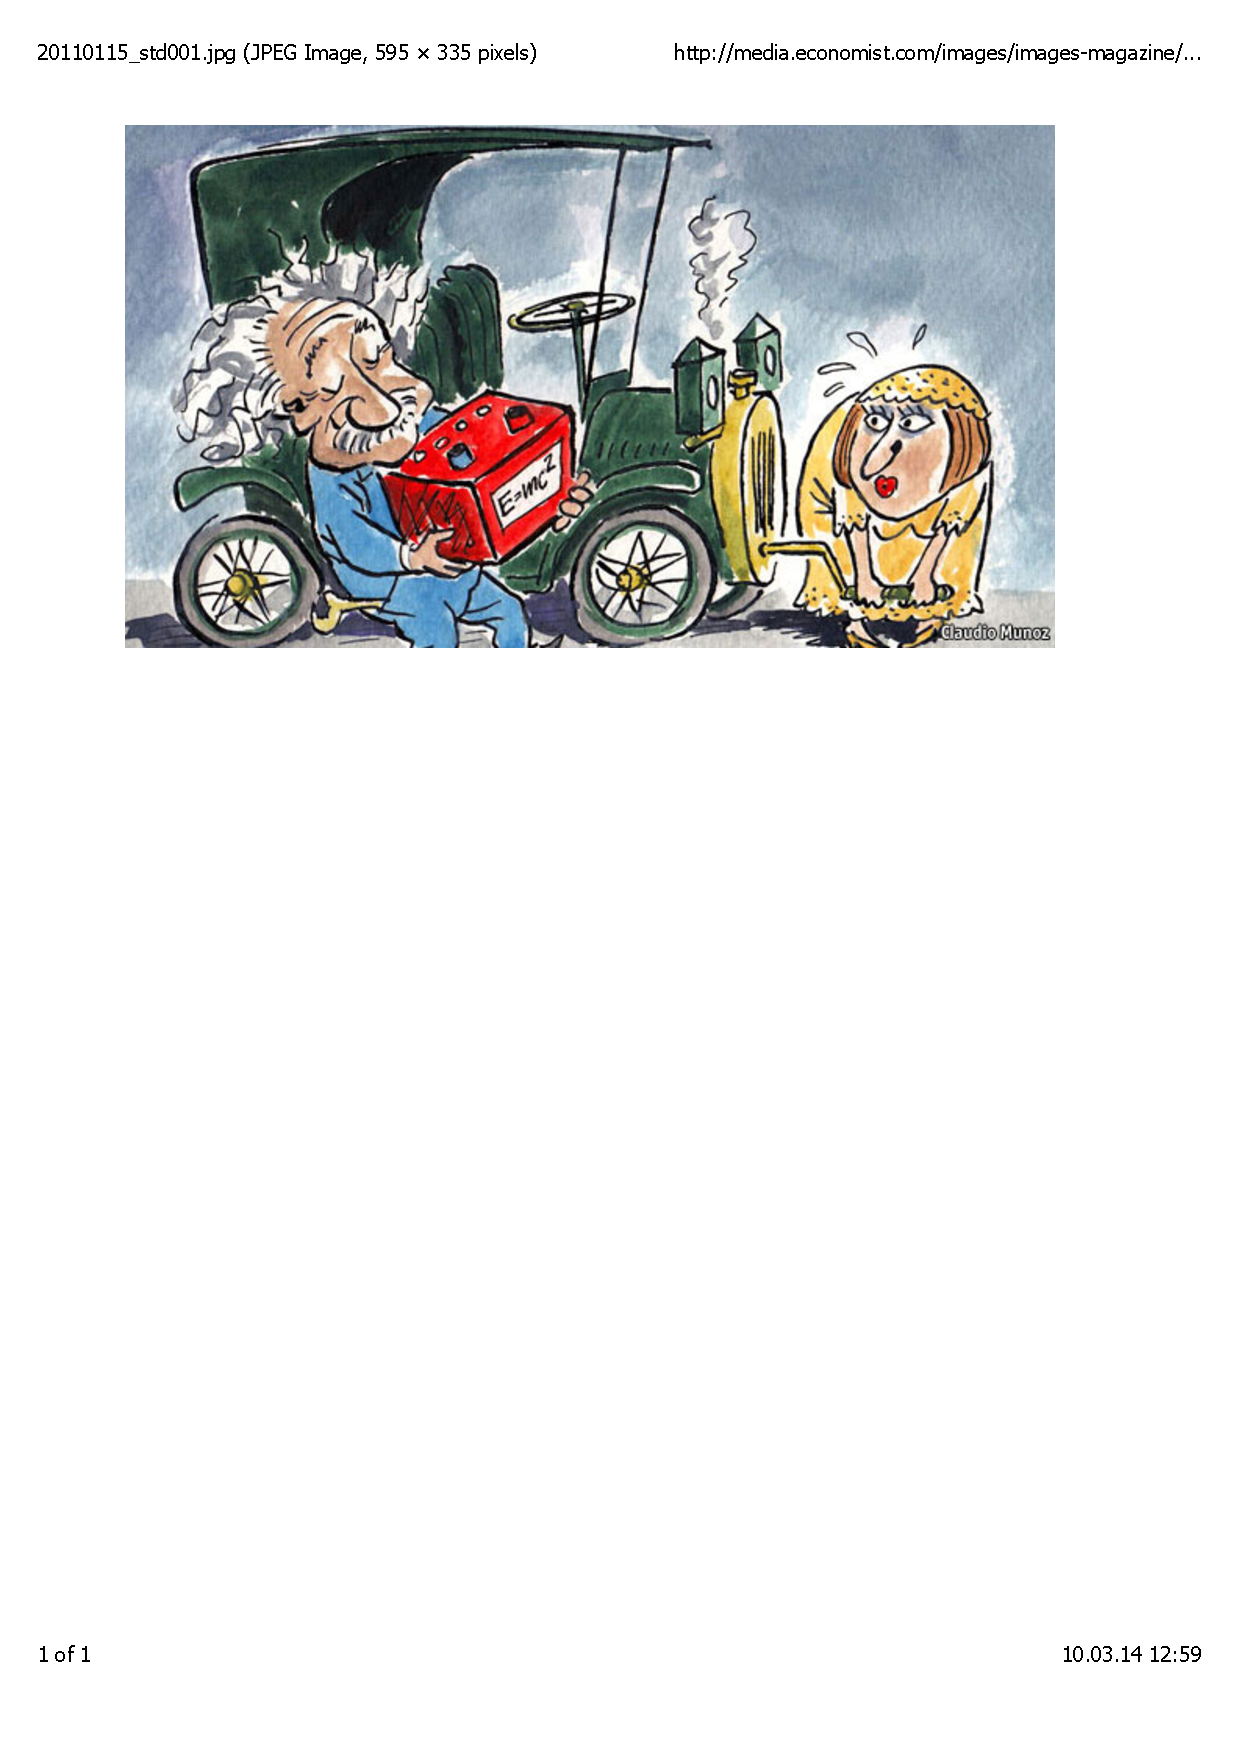
\includegraphics[viewport = 60 530 510 790, clip, scale=0.3]{figures/economist.pdf}
    \end{column}
    \end{columns}
\end{frame}

\begin{frame}
    \frametitle{Aurora borealis}
    \begin{columns}
    \begin{column}{.50\textwidth}
	\ \\
    \end{column}
    \begin{column}{.50\textwidth}
	\centering
	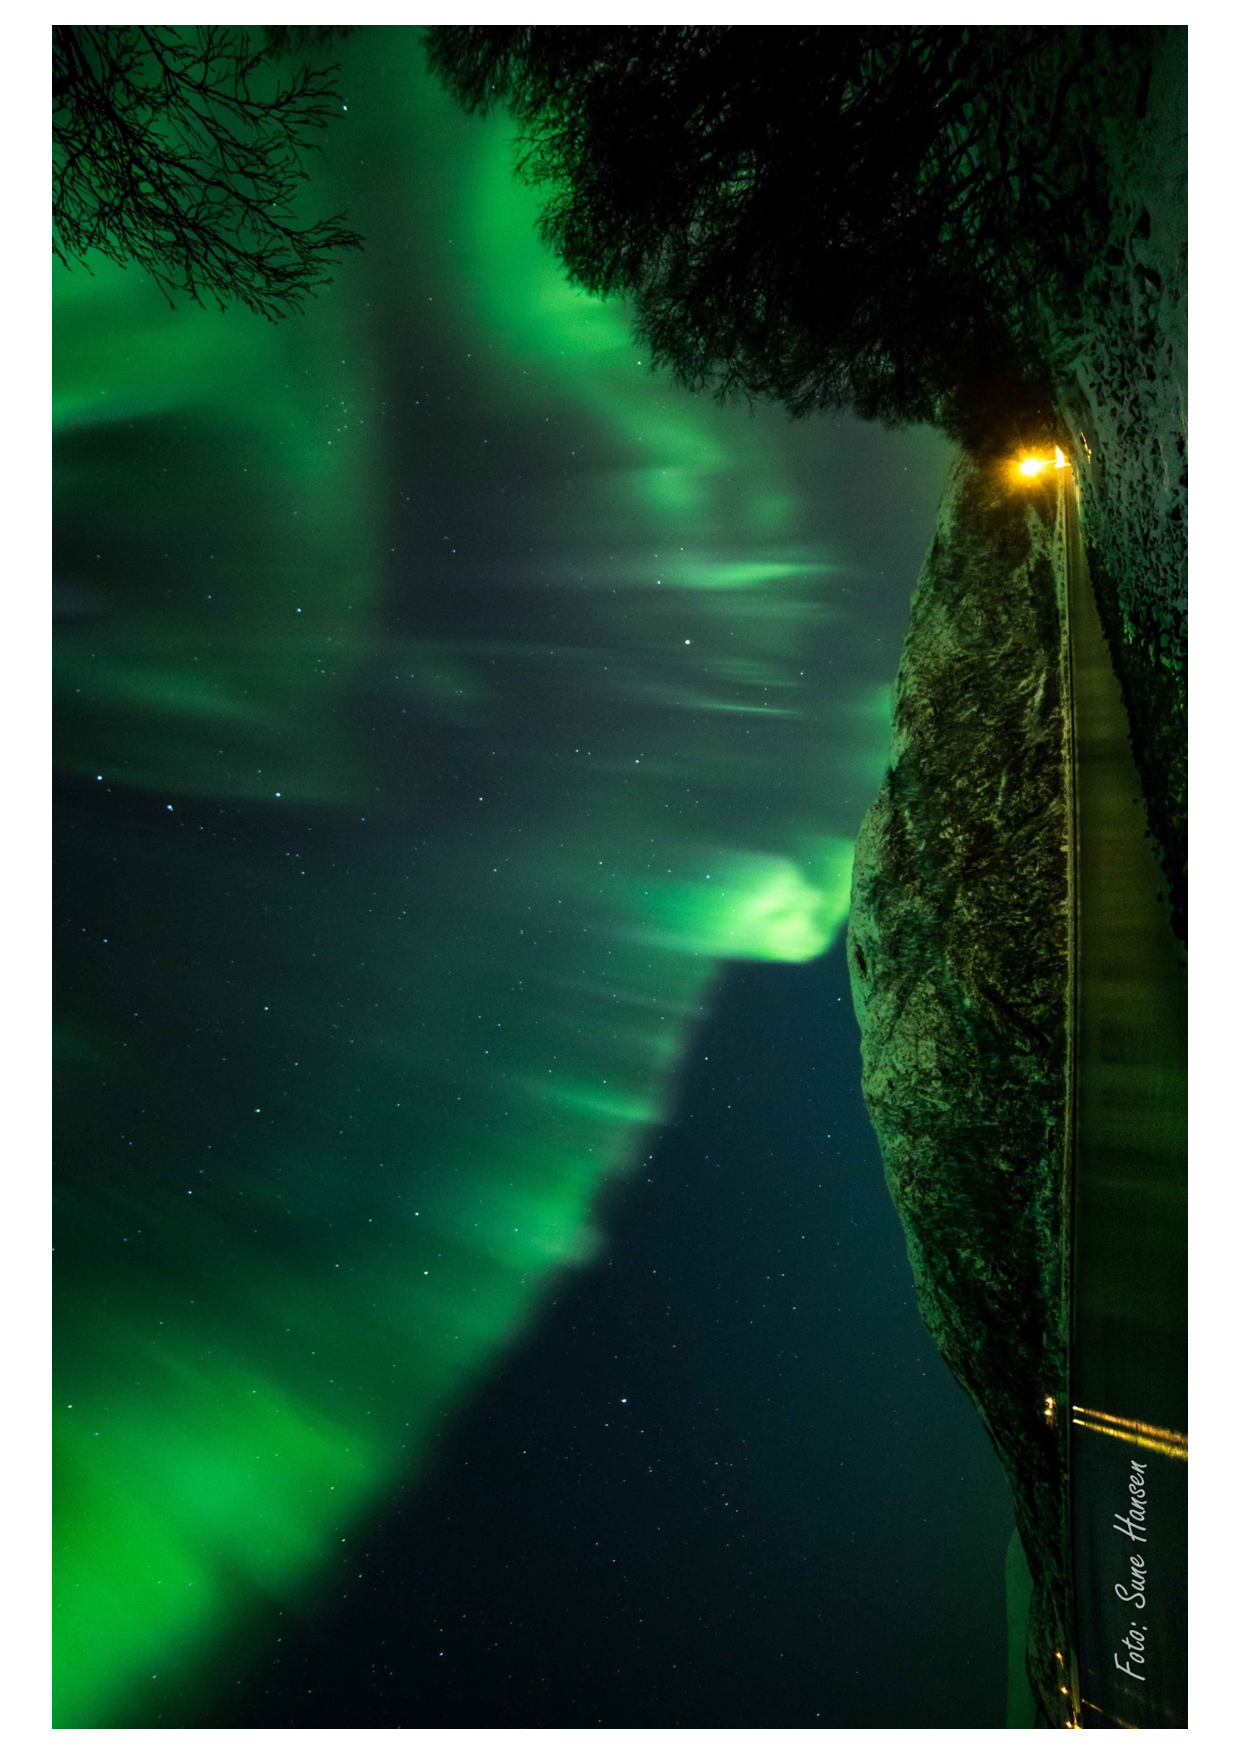
\includegraphics[viewport = 0 0 600 800, clip, scale=0.15, angle = -90]{figures/aurora.pdf}
    \end{column}
    \end{columns}
\end{frame}

\begin{frame}
    \frametitle{Summary}
\end{frame}


\end{document}
